\documentclass{article}

% -------------------- Packages --------------------
\usepackage{graphicx} % Required for inserting images
\usepackage{tabularx}
\usepackage{booktabs}
\usepackage[mode=text]{siunitx}
\usepackage{csquotes}\MakeOuterQuote{"}
\usepackage{xcolor}
\usepackage[
  colorlinks=true,
  linkcolor=blue,
  citecolor=blue,
  urlcolor=blue
]{hyperref}
\usepackage{soul}
\usepackage{placeins}
\usepackage[a4paper, margin=2.5cm]{geometry}
\usepackage{authblk}
\usepackage{booktabs}
\usepackage{tabularx}
\usepackage{dcolumn}
\usepackage{amsmath}
\usepackage{amssymb}
\usepackage{amsthm}
\theoremstyle{plain}
\newtheorem{proposition}{Proposition}
\newtheorem{corollary}{Corollary}
\usepackage{array}
\usepackage{threeparttable}
\usepackage{rotating}
\usepackage{tikz}
\usetikzlibrary{arrows.meta,positioning}
\newcolumntype{R}{>{\raggedleft\arraybackslash}X}

% -------------------- Bibliography --------------------
\usepackage[style=apa6,sortcites=true,sorting=nyt,backend=biber]{biblatex}
\addbibresource{references.bib}

\title{The Information Costs of Climate Misinformation: \\\large Evidence from Global Financial Data}
\ifdefined\AuthorVersion
\author[1]{James Rice}
\affil[1]{Department of Government, University of Essex}
\else
\author{}
\fi
\date{}

\begin{document}
\maketitle

\begin{abstract}

Climate misinformation can alter the information environment in which investors and liquidity providers trade. This paper examines that relationship in a panel of 204 listed climate-transition securities, using sector-specific exposure constructed from 217,954 English-language Facebook climate posts classified against nine energy sub-industries. Greater exposure is positively associated with quoted bid--ask spreads under monthly and local market-day controls. On a common sample of 486,655 security-days, the market-day estimate is $+0.0129$ percentage points per index point ($p=0.033$ under sector/date clustering), a pattern consistent with information-verification costs. The association changes sign and is imprecise after sector-month conditions are absorbed; with prior-session financial controls, the estimate is $-0.0014$ ($p=0.533$). Timing and alternative-outcome checks do not establish an additional robust response. The findings connect the political production of climate misinformation to the trading environment of energy equities while locating the positive spread association in shared sector conditions. The contribution is a sector-sensitive measure and a transparent account of where the liquidity association is observed, rather than a causal estimate of misinformation costs.
\end{abstract}

\noindent\textbf{Keywords:} Climate Misinformation, Information Asymmetry, Market Microstructure, Environmental Communication, Politics and Governance, Corporate Responsibility.

\section{Introduction}

The information landscape surrounding climate change has been systematically distorted by misinformation campaigns (\cite{cobb2025politics}). Markets aggregate information, but they do so at a price. Climate misinformation is produced for political ends---funded by fossil-fuel interests, amplified by ideologically motivated actors, and timed to political events (\cite{farrell2016network}; \cite{oreskes2010merchants}; \cite{cinelli2021echo})---yet market-microstructure theory gives two opposing predictions for its effect on trading costs. If misinformation increases the advantage of sophisticated traders who can distinguish credible signals from false ones, liquidity providers should widen bid--ask spreads to protect themselves. If misinformation instead attracts uninformed retail trading, the perceived share of informed order flow may fall and spreads may narrow even as the market's capacity to absorb informed trading deteriorates. Which pattern prevails is the central question of this paper.

This question connects two related literatures. Political-behavior research shows that misinformation changes beliefs, trust, and collective action (\cite{flynn2017misperceptions}; \cite{bursztyn2020misinformation}), while climate-finance research shows that climate news, disclosure, and policy uncertainty are priced in financial markets (\cite{engle2020hedging}; \cite{bolton2021climate}; \cite{pankratz2023climate}). Neither literature traces the daily flow of politically produced climate misinformation into the mechanism that sets trading costs. Market microstructure provides that link because the quoted bid--ask spread is an observable price of information asymmetry and a direct measure of market liquidity (\cite{GlostenMilgrom1985}; \cite{EasleyOHara1992}).

The theory distinguishes two competing channels. Under adverse selection, false claims about climate science, carbon policy, and the viability of low-carbon technologies make the implications for fossil-fuel and renewable firms harder to assess. Traders able to verify those claims gain an informational advantage over those who cannot. Liquidity providers then face greater expected losses when trading climate-transition equities with better-informed counterparties and may widen spreads. Under liquidity fragility, viral climate-policy and energy narratives instead draw noise traders into the affected sub-industries, potentially narrowing spreads as the uninformed share rises. H1 tests the narrowing-spread prediction. Section~\ref{sec:theory} develops the mechanisms and distinguishes their theoretical implications from the information available in daily quote data.

The empirical analysis starts with 726,890 security-day observations on 204 listed climate-transition securities, representing 198 distinct company names, from January 2012 to December 2025. Financial estimation is restricted to the content index's observed window, January 2012--October 2025. The primary outcome is the percent quoted bid--ask spread. The exposure measure is constructed by classifying 217,954 English-language Facebook climate posts from the Meta Content Library against nine TRBC energy sub-industries. Each security inherits its sub-industry's exposure on each date, producing within-day cross-sectional variation while preserving the political and economic content of the posts. Correctly mapped listing-market effects, sector-month controls and prior-session characteristics assess how locally the spread association can be identified.

Greater sector-specific misinformation exposure is positively associated with quoted spreads in the monthly and local market-day specifications. The latter coefficient is $+0.0129$ ($p=0.033$ under sector/date clustering), supporting the view that the climate-information environment and trading costs move together. This positive association is not stable after sector-month conditions are absorbed: on the same sample the coefficient becomes $-0.0033$ ($p=0.117$), and the prior-session-control specification yields $-0.0014$ ($p=0.533$). The evidence therefore identifies a positive association in the broader sector information environment while placing a clear boundary on a daily misinformation-specific interpretation. The null estimates are part of that finding, rather than evidence that climate misinformation is financially irrelevant.

The paper makes three contributions. First, it extends market-microstructure theory to politically produced climate misinformation and makes the competing adverse-selection and participation predictions explicit. Second, it provides a high-frequency sector-sensitive exposure measure that maps political misinformation to the sub-industries whose values depend on the contested information. Third, it shows that a positive association remains after local market-day conditions are absorbed, while sector-month controls materially change the identifying comparison. Together, these contributions connect the political production of misinformation to the liquidity of climate-transition equities and clarify which part of the relationship the observational evidence supports.

The rest of the paper proceeds as follows. Section~\ref{sec:lit_review} reviews research on information and market liquidity and connects it to climate misinformation in financial markets. Section~\ref{sec:theory} develops the competing adverse-selection and liquidity-fragility mechanisms and states the hypothesis formally. Section~\ref{sec:data} introduces the firm-day financial panel and misinformation corpus. Section~\ref{sec:model} separates the market-liquidity design from the benchmark risk-and-return designs and sets out the identification and inference strategy. Section~\ref{sec:results} reports the main estimates, relevance checks, and robustness comparisons. Section~\ref{sec:discussion} interprets the findings, and Section~\ref{sec:conclusion} concludes.

\section{Literature Review}
\label{sec:lit_review}

\subsection{Information and Market Liquidity}

Market liquidity depends on the distribution and credibility of information. When some traders possess information that others lack, liquidity providers face the risk of trading at stale prices with better-informed counterparties (\cite{Akerlof1970}; \cite{GlostenMilgrom1985}; \cite{EasleyOHara1992}; \cite{Kyle1985}). They recover the expected loss through the bid--ask spread, while price impact records how strongly order flow moves prices. These measures make the trading-cost implications of information asymmetry observable. Costly information prevents markets from becoming fully efficient (\cite{GrossmanStiglitz1980}; \cite{Stiglitz2000}), and liquidity providers revise quotes as the perceived composition of informed and uninformed order flow changes (\cite{Hasbrouck1991}; \cite{easley1996}). Wider spreads indicate lower market liquidity and can pass through to firms' costs of capital (\cite{Tse2024}; \cite{Aliyev2025}; \cite{Aquilina2025}).

The credibility of public signals shapes this information environment. Financial disclosure lowers the cost of acquiring reliable information when investors regard the discloser as credible; weak or non-credible signals raise verification costs and the cost of capital (\cite{DiamondVerrecchia1991}; \cite{Verrecchia2001}; \cite{healy2001information}; \cite{LeuzVerrecchia2000}; \cite{BushmanSmith2001}; \cite{GoldsteinYang2017}). Investors' updates also depend on the perceived bias and authenticity of the source (\cite{Dye1985}; \cite{Cologna2022ValueJudgements}; \cite{KorehMandelkern2024}). Misinformation can therefore affect liquidity without changing firms' underlying cash flows: it degrades the public signal, increases the cost of separating credible information from false claims, and changes the risk that liquidity providers attach to incoming orders. Recent studies linking digital information and misinformation to liquidity document related effects on market microstructure (\cite{HerzingMuck2025}; \cite{DeesOzyurtMiller2026}; \cite{Mo2026ClimateRiskDisclosureMispricing}; \cite{LEIPPOLD202264}).

\subsection{Climate Misinformation and Financial Markets}

Climate misinformation is a politically produced distortion of that public signal. Organized campaigns by carbon-intensive industries have manufactured uncertainty about climate science and regulation, while partisan media and digital platforms amplify the resulting claims (\cite{oreskes2010merchants}; \cite{farrell2015corporate}; \cite{farrell2016network}; \cite{SupranRahmstorfOreskes2023}; \cite{VosoughiRoyAral2018}; \cite{acemoglu2010spread}). Exposure changes factual beliefs, hardens partisan misperceptions, erodes trust, and resists correction (\cite{flynn2017misperceptions}; \cite{NyhanReifler2010}; \cite{lewandowsky2017beyond}; \cite{bursztyn2020misinformation}; \cite{lazer2018science}; \cite{cobb2025politics}). Climate misinformation is a political problem because it distorts the evidence citizens use to evaluate policy proposals and hold decision-makers accountable. Organized interests can exploit uncertainty about climate science to weaken support for mitigation and delay regulation (\cite{farrell2019misinfo}). Understanding climate change requires interpreting long-term trends and probabilistic evidence; misleading arguments can exploit that difficulty by treating a cold weather event as a refutation of warming or uncertainty as evidence that action is unnecessary. \textcite{CookEllertonKinkead2018} show how such claims rely on faulty premises and reasoning. Confusion therefore need not reflect a simple absence of information: apparently plausible arguments and trusted partisan sources can make false claims persuasive. These studies establish the political and behavioral consequences of misinformation, but they do not show how the same content affects the liquidity of firms whose values depend on climate policy.

For businesses, these distortions can cloud expectations about regulation, demand for low-carbon products, and the returns to long-lived investments. That connection is plausible because climate-transition firms are unusually exposed to contested political information. Subsidies, carbon prices, disclosure requirements, and phase-out timetables are set through political institutions and international negotiations. Political and policy uncertainty carries a risk premium and raises volatility (\cite{PastorVeronesi2012}; \cite{PastorVeronesi2013}; \cite{BakerBloomDavis2016}), while partisan information and market sentiment can move prices independently of fundamentals (\cite{AZZIMONTI2023}; \cite{lei2023political}; \cite{DeLongShleiferSummersWaldmann1990}). Climate risk, news, and disclosure are likewise reflected in carbon premia, green-bond pricing, divestment, and institutional holdings (\cite{engle2020hedging}; \cite{bolton2021climate}; \cite{HongLiXu2019}; \cite{pankratz2023climate}; \cite{KruegerSautnerTangZhong2024}; \cite{flammer2021corporate}; \cite{FriedeBuschBassen2015}; \cite{Drahos_2025}). Misinformation differs from ordinary policy uncertainty because it corrupts the signal investors use to evaluate these exposures.

The verification problem is especially salient in fragmented climate governance, where public rules, transnational networks, private standards, taxonomies, and ratings offer competing signals whose authority can be politically contested or vulnerable to capture (\cite{KeohaneVictor2011}; \cite{HaleHeld2018}; \cite{Bodansky2016}; \cite{Rajamani2017}; \cite{AbbottSnidal2000}; \cite{ButheMattli2011}). Misinformation then makes genuine sustainability information harder to distinguish from greenwashing (\cite{delmas2011drivers}; \cite{marquis2016scrutiny}). The unresolved question is whether politically produced climate misinformation changes the trading costs through which markets process that information. The next section derives the competing liquidity predictions.

\section{Theory: Climate Misinformation and Market Liquidity}
\label{sec:theory}

The theoretical construct is information asymmetry: one party holds material information that another lacks (\cite{Akerlof1970}; \cite{Stiglitz2000}; \cite{StiglitzKosenko2024a}; \cite{StiglitzKosenko2024b}). The primary dependent variable is not information asymmetry itself, but the firm-day percent quoted bid--ask spread used to observe its liquidity consequences. In the sequential-trade model of \textcite{GlostenMilgrom1985}, a market maker posts a bid and an ask without knowing whether the next order comes from an informed or an uninformed trader. The spread compensates for expected losses to informed counterparties: the greater the perceived informed-trading risk, the wider the quote required to break even (\cite{EasleyOHara1992}; \cite{Hasbrouck1991}). A wider spread indicates lower quoted liquidity and is consistent with greater adverse-selection pressure, although it can also reflect inventory risk and other trading costs.

Climate misinformation changes the public signal that investors use to value climate-exposed firms. Subsidy regimes, carbon prices, and regulatory timetables are political outcomes, and misinformation makes claims about those outcomes harder to evaluate (\cite{PastorVeronesi2012}; \cite{PastorVeronesi2013}; \cite{delmas2011drivers}; \cite{marquis2016scrutiny}). Investors differ in their ability and willingness to verify these signals. The resulting heterogeneity can affect trading through two competing microstructure channels.

Under the adverse-selection channel, sophisticated investors are better able to identify the credible climate-pricing signal, while less-informed investors are more likely to trade on false claims. This divergence increases the informational advantage of sophisticated traders. A liquidity provider who expects greater losses when orders originate from better-informed counterparties widens the bid--ask spread and quotes less depth. Per-dollar price impact should move in the same direction because trades reveal more private information. The observable prediction is therefore wider spreads and higher price impact, both indicating lower liquidity (\cite{grossman1980impossibility}; \cite{chordia2000commonality}; \cite{Han2022}; \cite{bordalo2020}). Here, sophistication refers to investors' capacity to verify information, not to a firm's climate performance. Larger or wealthier firms may nevertheless have better disclosure, stronger compliance capacity, and a more informed investor base, jointly affecting misinformation exposure and liquidity. Firm fixed effects and the market-capitalization control address stable firm differences and observed size changes, but do not eliminate time-varying differences in disclosure quality or regulatory preparedness. Figure~\ref{fig:theory_paths} summarizes the proposed adverse-selection pathway.

Under the liquidity-fragility channel, viral misinformation may divert attention from accurate information and attract inexperienced retail traders into climate-exposed stocks (\cite{barber2008all}; \cite{PengXiong2006}; \cite{sims2003}). If the uninformed share rises, the market maker's perceived probability that the next order is informed falls, narrowing the quoted spread. Yet this new order flow is shallow and noisy: each additional dollar traded moves the price by more, increasing price impact and weakening price efficiency. Liquidity fragility is this joint state in which trading appears cheaper at the quoted spread while the market's capacity to absorb informed flow deteriorates.

\begin{figure}[htbp]
\centering
\definecolor{pathnavy}{HTML}{173B57}
\definecolor{pathblue}{HTML}{EAF2F7}
\definecolor{pathgold}{HTML}{D8A547}
\definecolor{pathink}{HTML}{243746}
\begin{tikzpicture}[
  stage/.style={
    draw=pathnavy!60,
    fill=pathblue,
    rounded corners=2.2mm,
    align=center,
    text width=2.80cm,
    minimum height=2.65cm,
    inner xsep=2.5mm,
    inner ysep=3mm,
    font=\footnotesize,
    text=pathink
  },
  shock/.style={
    stage,
    draw=pathgold!85!black,
    fill=pathgold!14
  },
  outcome/.style={
    stage,
    draw=pathnavy,
    fill=pathnavy,
    text=white
  },
  flow/.style={
    -{Latex[length=2.5mm,width=1.7mm]},
    draw=pathgold!85!black,
    line width=0.9pt
  },
  node distance=0.42cm
]
\node[shock] (misinfo) {
  {\tiny\bfseries\color{pathgold!55!black}INFORMATION\\SHOCK}\\[4pt]
  \textbf{\mbox{Sector-specific}\\climate\\misinformation}
};

\node[stage, right=of misinfo] (signal) {
  {\tiny\bfseries\color{pathnavy!72}PUBLIC\\SIGNAL}\\[4pt]
  \mbox{Credible signals}\\\mbox{become harder and}\\\mbox{costlier to verify}
};

\node[stage, right=of signal] (risk) {
  {\tiny\bfseries\color{pathnavy!72}ADVERSE-SELECTION\\RISK}\\[4pt]
  \mbox{Liquidity providers}\\\mbox{expect greater losses}\\\mbox{to informed traders}
};

\node[outcome, right=of risk] (liquidity) {
  {\tiny\bfseries\color{pathgold!65}LIQUIDITY\\RESPONSE}\\[4pt]
  \mbox{Quoted bid--ask}\\\mbox{spreads widen and}\\\mbox{market liquidity falls}
};

\draw[flow] (misinfo) -- (signal);
\draw[flow] (signal) -- (risk);
\draw[flow] (risk) -- (liquidity);
\end{tikzpicture}
\caption{The adverse-selection pathway linking sector-specific climate misinformation to market liquidity.}
\label{fig:theory_paths}
\end{figure}

The first two pathways imply different signs for the spread response. Adverse selection predicts wider quotes, whereas liquidity fragility predicts narrower quotes alongside weaker capacity to absorb informed trading. H1 therefore states that \emph{higher security-day exposure to sector-specific climate misinformation is associated with narrower percent quoted spreads.} The statistical test uses the sign and precision of the spread coefficient across increasingly local comparisons. The positive coefficient in a baseline specification counts against H1 in that specification; an imprecise coefficient in a more saturated model does not justify a general rejection. The daily VWAP--midquote gap is examined as a complementary price-dispersion measure, but does not measure per-dollar transaction price impact and cannot complete a joint mechanism test.

Rolling CAPM beta and Fama--French five-factor excess returns provide benchmark outcomes rather than alternative measures of liquidity (\cite{DeLongShleiferSummersWaldmann1990}; \cite{PastorVeronesi2012}). The climate-finance literature implies that financial responses depend on which climate news and disagreement is relevant to a security (\cite{engle2020hedging}; \cite{bolton2021climate}; \cite{HongLiXu2019}; \cite{pankratz2023climate}). Their interpretation also depends on an appropriate regional factor mapping. The supplied factor-derived outcomes are retained as descriptive diagnostics, with their mapping limitation stated explicitly; they are not used to establish changes in systematic risk or return premia. Liquidity, timing and sector-condition comparisons supply the substantive empirical tests.

\section{Data}
\label{sec:data}

The unit of analysis is the security-day. The financial input contains 726,890 observations on 204 listed climate-transition securities from January 2012 to December 2025. These securities---fossil-fuel incumbents and renewable challengers---are selected from a broader 19,183,738-security-day universe using nine TRBC energy sub-industries. The financial panel supplies daily quotes, trading characteristics and descriptive risk-and-return variables from Refinitiv Workspace, FRED, the World Bank and the Kenneth French Data Library. The climate-misinformation corpus supplies the 217,954 unique English-language Facebook posts used to construct the exposure measure. The observed index covers 3 January 2012--13 October 2025, and dates outside that support are excluded rather than coded as unexposed. Appendix Tables~\ref{tab:panel_g}--\ref{tab:panel_n} and~\ref{tab:qwen_type} describe the corpus and its classifications. Appendix Tables~\ref{tab:panel_a}--\ref{tab:panel_f} document the supplied financial assembly, while the estimation-sample tables distinguish those inputs from the complete-case regressions. Processing is implemented in Python, following the transparency principles of \textcite{ChristensenMiguel2018}.

\subsection{Financial Panel and Outcome Measures}
\label{sec:data_financial}

The financial data come from a panel of 204 listed climate-transition securities sourced from Refinitiv Workspace via the Eikon Python API. The sample is defined by membership in nine TRBC energy sub-industries spanning the fossil-fuel value chain (Coal, Integrated Oil \& Gas, Oil \& Gas Drilling, Oil \& Gas Exploration and Production, Oil \& Gas Refining and Marketing, Oil \& Gas Transportation Services, Oil Related Services and Equipment) and the renewable transition (Renewable Energy Equipment \& Services, Renewable Fuels). Actual listing markets include mainland China, Hong Kong, Taiwan, Japan, Indonesia, Malaysia, Brazil, the United States, the United Kingdom, France, Germany and the Netherlands. Security identifiers are kept distinct: multiple share classes and cross-listings do not become independent firms. Daily prices, volume, turnover, capitalization, dividends, bid--ask quotes and VWAP describe the trading environment (\cite{Karpoff1987}; \cite{Parkinson1980}). The percent quoted spread is the bid--ask difference divided by the quote midpoint and expressed in percent. It is the primary liquidity outcome; it does not identify effective execution costs or the private-information component of the spread on its own.

One practical concern is timing. The Shanghai trading day ends before the New York session begins, so a same-date merge can associate posts made after an Asian close with that day's quotes. The timing checks distinguish the previous calendar day from the previous observed session with positive volume and a positive close. Session lags are formed before selecting complete cases on the spread, and source dates outside the corpus window or gaps exceeding ten calendar days are excluded. Static characteristics are merged by security. Listing market is assigned using the exchange suffix of the RIC, separating, for example, Indonesian .JK, Brazilian .SA and Taiwanese .TW listings from US and Japanese markets. The complete market crosswalk accompanies the replication materials. This assignment supplies the local market-day fixed effects, while headquarters country remains a separate characteristic.

The financial input also contains regional macroeconomic series from FRED and the World Bank: GDP growth, the supplied unemployment-labelled series, and CPI inflation (\cite{FederalReserveBankofStLouis2025}; \cite{WorldBank2025}). These are carried forward from lower-frequency observations (\cite{StockWatson2008}):
\begin{equation}
M_{r,d}=M_{r,q(d)},\qquad q(d)=\max\{q:\mathrm{start}(q)\leq d\}.
\end{equation}
The supplied region groups are not equivalent to actual listing markets. The substantive spread specifications therefore use market-day effects instead of relying on this regional macro mapping. In particular, the unemployment-labelled input is documented without assigning it a structural unemployment interpretation.

Daily Fama--French five-factor returns---market excess return (MktRF), size (SMB), value (HML), profitability (RMW), and investment (CMA)---are supplied from the Kenneth French Data Library.\footnote{Data available at \url{https://mba.tuck.dartmouth.edu/pages/faculty/ken.french/data_library.html}.} The input includes regional factors and corresponding risk-free rates. Their descriptive coverage is reported in the appendix. Factor-derived outcomes require a correct association between each security and its relevant market. They are therefore retained as supplied-data benchmarks, with no claim that correcting a fixed-effect market label reconstructs a valid risk-free-rate series or regional factor exposure.

Three variables are constructed from the raw panel. The daily simple return is
\begin{equation}
R_{i,t} = \frac{P_{i,t} - P_{i,t-1}}{P_{i,t-1}} \times 100,
\end{equation}
where $P_{i,t}$ is the closing price of firm $i$ on day $t$. The daily excess return is $R^e_{i,t} = R_{i,t} - R_{f,t}$, where $R_{f,t}$ is the regional daily risk-free rate from the Fama--French data. The rolling CAPM beta comes from 252-trading-day rolling OLS regressions of firm excess returns on the regional market excess return, requiring a minimum of 126 observations per window:
\begin{equation}
\hat{\beta}_{i,t} = \frac{\text{Cov}(R^e_{i,s}, \text{MktRF}_s)}{\text{Var}(\text{MktRF}_s)}, \quad s \in [t-251, t].
\end{equation}

The rolling beta is a slow-moving measure by construction, and thin or non-synchronous trading can bias a conventional OLS beta (\cite{ScholesWilliams1977}; \cite{Dimson1979}). These issues matter alongside market matching: a low estimated beta need not imply low fundamental climate risk. Appendix Table~\ref{tab:beta_region_mktcap} reports supplied betas by stored region group and capitalization quintile as a description of the input. Since those groups do not identify actual listing markets, neither their differences nor the factor-derived regression coefficients establish cross-country differences in systematic risk. The quoted-spread analysis instead uses directly observed quotes and separately assigned market-day effects.

The merged climate-transition panel is uniquely indexed by security and date, with no duplicates. Mainland China and Indonesia contribute the largest security counts, followed by the United States. Appendix Table~\ref{tab:energy_desc_coverage} documents the full financial input; Table~\ref{tab:markets} reports actual listing markets in the 485,800-observation prior-control sample, while the nested contemporaneous-control comparison has 486,655 observations. The prior-control sample contains 202 securities and 197 distinct company names. Missing quotes, nonpositive trading activity and required financial controls determine complete-case coverage. Retaining a long calendar panel does not itself eliminate survivorship or selection concerns.

Finally, the climate-transition panel is merged on calendar date and firm sub-industry with the firm-day misinformation-exposure index built from the Meta Content Library, described in Sections~\ref{sec:data_misinfo} and~\ref{sec:LLM} below. The main regressions use $\mathrm{Exp}^{\text{mean}}_{i,t}$ as the headline regressor of interest, with $\log(1+\mathrm{Exp}^{\text{sum}}_{i,t})$, $M^{\text{mean}}_{i,t}$, and $R^{\text{mean}}_{i,t}$ as variant specifications, all defined in Section~\ref{sec:LLM}.

\subsection{Climate Misinformation Corpus}
\label{sec:data_misinfo}

The misinformation measure is built from 217,954 unique English-language public Facebook posts---the subset of a 265,652-post corpus extracted from the Meta Content Library (MCL) whose Meta-recorded creation date matches at least one trading day in the climate-transition panel. The corpus was assembled through keyword searches across eight thematic datasets covering climate adaptation, climate politics, global climate justice, resilience, climate activism, and ecological themes; the posts span December 2009 to October 2025 and come from a long-tailed distribution of pages and profiles. Each post carries platform-reported engagement counts---likes, shares, comments, total reactions, and views---plus metadata on content type, surface type, and owner characteristics. Appendix Table~\ref{tab:panel_g} reports summary statistics on the corpus as a whole.

The corpus is an English-language, keyword-selected sample of public content, not a representative sample of national Facebook use. The available summaries do not establish the countries of origin of posts or the geographic distribution of their audiences, so differences in platform access, language, and user composition cannot be separated from differences in misinformation production. The exposure measure instead treats Facebook as a potential transnational information environment: claims about energy technologies, carbon policy, or fossil-fuel demand can circulate across borders and inform investors trading firms in the same sub-industry. For example, a claim originating in India could matter for a French-listed company if it reaches that company's investors or concerns markets or technologies relevant to its cash flows. The link is shared sector relevance and possible cross-border circulation, not the automatic transmission of every foreign post to every firm. The index measures the availability of relevant content, rather than observed investor attention or a country-to-country transmission effect.

The corpus enters this paper at the level of individual posts. Each (post, sub-industry) pair is scored by a single large language model on two continuous 0--100 scales---sector relevance and climate-or-energy misinformation---as described in Section~\ref{sec:LLM}; the firm-day index used in the empirical models is built from those scores. Three properties of the corpus matter for the analysis. First, the corpus is heavy-tailed in volume by year, with English-language climate-post volume more than tripling after 2019 (Appendix Table~\ref{tab:panel_j}). Second, the corpus is concentrated in supply: a small set of high-volume pages and profiles produces a large share of total posts (Appendix Table~\ref{tab:panel_l}), and platform-reported engagement counts are themselves heavy-tailed, with the highest-engagement posts diffusing on the order of three times the mean shares of the median post---a pattern consistent with the finding that misleading content travels disproportionately (\cite{VosoughiRoyAral2018}). Third, the corpus mixes climate-scientific content, climate-political content, and climate-adjacent content that is on-topic for some sub-industries and entirely off-topic for others; the firm-day construction in Section~\ref{sec:LLM} is what makes the sub-industry partition operational.

The classifier uses an open-weight model, and the post-level classifications and firm-day index built from them are released with the replication package. The raw post text falls under the MCL terms of use and is not redistributed. The classifier is assessed with a rubric-development spot-check (Section~\ref{sec:LLM}), which informed the rubric and is not an independent held-out or hand-coded gold-standard sample (\cite{grimmer2022text}). Constructing a gold standard is less straightforward than for a binary label because the task requires two continuous 0--100 judgments---sector relevance and climate-or-energy misinformation---over nuanced content. A hand-coded benchmark would nevertheless provide a valuable direction for further measurement validation.

\subsection{LLM Classification of Misinformation}
\label{sec:LLM}

This section describes the classification framework that turns the corpus into a firm-day measure of misinformation exposure (\cite{WardleDerakhshan2017}). The design goal follows directly from the inference problem in Section~\ref{sec:model}: a regressor that is to vary across firms within a calendar day must be built by asking, for every post, a separate question of every sub-industry the panel contains. That is what the classifier does. It is called once on each of the 1,959,707 (post, sub-industry) pairs---covering the nine TRBC energy sub-industries and 217,954 posts with valid output---and returns, for each pair, how relevant the post is to that sub-industry and how much climate-or-energy misinformation it contains. A market-wide daily index that collapsed a model's per-post scores into one number would, by construction, assign every firm the same value on a given day and reinstate the firm-invariant problem this paper is designed to avoid; only the per-sub-industry judgment produces the cross-sectional variation the design needs.

A single high-capacity model is used rather than an ensemble. At 1.96 million judgments, the 35-billion-parameter model is tasked with distinguishing sincere false claims from satire and sector-relevant claims from off-topic content using one explicit rubric. Independent human annotation remains necessary to quantify classification accuracy. Automated detection systems are themselves vulnerable to adversarial manipulation and raise ethical concerns (\cite{QiuLiuZhou&Huang2022}; \cite{HorneNevo&Smith2023}), so the design relies on one locally hosted classifier with fixed decoding settings and persisted outputs and whose rubric is fixed in advance and made explicit below.

The model is \texttt{Qwen3.6-35B-A3B-FP8}, a mixture-of-experts model with 35 billion total parameters and approximately 3 billion active parameters per token, served in 8-bit floating-point precision using the vLLM 0.21 inference engine. Inference uses temperature zero and structured-JSON grammar enforcement via the \texttt{xgrammar} backend, with persisted structured outputs for each (post, sub-industry) judgment (\cite{westwood2025measuring}; \cite{gilardi2023chatgpt}; \cite{santurkar2023whose}). Each judgment receives the firm's sub-industry profile (industry name, the set of countries and listing regions of firms in that sub-industry, and a list of example firm names) and the post (text, date, content type, link-attachment caption and description). The rubric instructs the model to score two continuous 0--100 quantities: \emph{sector relevance} $R_{p,s}$, capturing how materially the post's content relates to firms in sub-industry $s$, and \emph{climate-or-energy misinformation} $M_{p,s}$, capturing the degree to which the post contains false, misleading, or pseudoscientific claims about climate science or energy.

Two features of the rubric matter. First, misinformation is bounded to climate or energy claims. A post that contains political conspiracy theories unrelated to climate---antisemitic content about EU politicians, anti-vaccination conspiracies, electoral fraud claims---scores $M_{p,s}=0$ regardless of how false those other claims are; the score is a measure of climate-misinformation exposure, not a general misinformation index. Second, satire and parody are bounded to be not misinformation. A sarcastic Facebook post mocking climate denial that begins ``MDPI, the predatory journal of which nothing can be believed, according to Facebook climate experts'' receives $M_{p,s}=0$ with the rationale ``satirical parody mocking climate denialism, not a sincere assertion of false claims''. These features were added to the rubric after a rubric-development spot-check on the first 2,000 judgments revealed that a default rubric over-scored political and parody content; the spot-check is reported in Appendix~\ref{sec:firmday_validation}.

The per-post composite exposure index is
\begin{equation}
\mathrm{Exp}_{p,s} \;=\; \frac{R_{p,s}\,M_{p,s}}{100},
\label{eq:exposure_post}
\end{equation}
on a 0--100 scale, which is non-zero only when the post is sector-relevant for sub-industry $s$ \emph{and} contains climate or energy misinformation. The product, rather than either factor alone, is the object of interest because the economic channel requires both: a false climate claim that has nothing to do with coal does not change what a coal trader needs to price, and an accurate, highly relevant post about coal carries no misinformation for the market to misprice. The index isolates the intersection---misinformation that is \emph{about} the firm's sector. The firm-day regressor used in the empirical models is the mean of this composite across the day's paired posts, evaluated at the firm's sub-industry:
\begin{equation}
\mathrm{Exp}^{\text{mean}}_{i,t} \;=\; \frac{1}{|P_t|}\sum_{p \in P_t} \mathrm{Exp}_{p,\,s(i)},
\label{eq:exposure_firmday}
\end{equation}
where $P_t$ contains the valid scored climate posts for the relevant sector whose Meta-recorded creation date matches calendar date $t$, and $s(i)$ is the TRBC sub-industry of firm $i$. Two volume-style variants enter the robustness checks: $\mathrm{Exp}^{\text{sum}}_{i,t}=\sum_p \mathrm{Exp}_{p,s(i)}$ (sensitive to the number of climate posts a firm's sector sees on a given day) and $\log(1+\mathrm{Exp}^{\text{sum}}_{i,t})$ (which tames the right skew). The raw components $R^{\text{mean}}_{i,t}$ and $M^{\text{mean}}_{i,t}$ are also persisted, to test whether the composite or one of its constituents carries the signal.

Three properties of the regressor matter for the inference design. First, two firms in different sub-industries on the same date receive different exposures: the model evaluates each post against the specific sub-industry, so a Renewable-Fuels firm and a Coal firm on the same trading day inherit different scores from the same set of posts. Second, two firms in the \emph{same} sub-industry on the same date share a value by construction; the level of aggregation at which the model is asked to reason is the sub-industry, not the firm. Firm-level fixed effects in the empirical models absorb the constant level of exposure that any firm experiences over the sample, leaving within-firm between-day variation as the identifying contrast. Third, the share of firm-days with exactly $\mathrm{Exp}^{\text{mean}}=0$ is $44\%$ in the climate-transition panel (Appendix Table~\ref{tab:v2_descriptive} and Appendix Figure~\ref{fig:v2_iv_distribution})---these are firm-days on which paired climate posts were either off-topic for the firm's sub-industry or contained no misinformation---so the regressor is sparse, and the volume variants in the robustness section capture how the number of paired posts mediates the response. A total of 398 of the 1,959,707 (post, sub-industry) judgments returned a parsing error after five retries (0.02\%) and are dropped from any downstream firm-day on which they would otherwise have entered the average.

\section{Empirical Strategy}
\label{sec:model}

The empirical strategy separates the main quoted-liquidity design from benchmark risk-and-return diagnostics. The baseline tests the spread prediction using within-security changes in the sector-specific misinformation index. A nested comparison then introduces daily and local market-day effects, followed by sector-month effects. These comparisons make the identifying variation explicit rather than allowing a change in sample to explain a coefficient difference. The factor-derived diagnostics remain secondary because the supplied regional mapping limits their financial interpretation.

\subsection{Design 1: Market Liquidity}
The baseline spread specification is:
\begin{equation}
\text{SpreadPercent}_{i,t}=\beta_1\mathrm{Exp}^{\mathrm{mean}}_{i,t}+\boldsymbol\gamma'\mathbf X_{i,t}+\alpha_i+\delta_{q(t)}+\varepsilon_{i,t}.
\label{eq:spread_reg}
\end{equation}
Here $\mathbf X_{i,t}$ contains log one plus trading volume, log market capitalization and the daily high--low price range divided by the closing price and expressed in percent. $\alpha_i$ denotes security fixed effects and $\delta_{q(t)}$ year-month effects. All logged variables are natural logarithms. Continuous financial controls and outcomes are winsorized at the first and ninety-ninth percentiles; exposure scores are not winsorized. The quoted spread is reconstructed as $200(A-B)/(A+B)$, where $A$ and $B$ are the daily ask and bid. Positive bid, non-crossed positive spread, positive volume and positive close are required.

The nested comparison replaces year-month effects first with calendar-date effects and then with listing-market-by-date effects. The latter absorb daily news, trading conditions and other shocks shared by securities in the same local market. All four contemporaneous-control specifications use the same 486,655 observations, controls and tail caps. The final nested specification adds sub-industry-by-month effects, separating daily exposure variation from the monthly information and valuation environment of the sector:
\begin{equation}
\text{SpreadPercent}_{i,t}=\beta_1\mathrm{Exp}^{\mathrm{mean}}_{i,t}+\boldsymbol\gamma'\mathbf X_{i,t}+\alpha_i+\lambda_{m(i),t}+\mu_{s(i),q(t)}+\varepsilon_{i,t}.
\label{eq:saturated}
\end{equation}
The fully conditional model additionally replaces contemporaneous financial controls with their values at the previous observed active trading session, denoted $\mathbf X_{i,t^-}$. This comparison uses 485,800 observations. It reduces direct conditioning on current trading activity, which may itself respond to the information environment, but does not make exposure exogenous. Its different control timing is shown separately from the common-sample nested comparison.

The companion price-dispersion outcome is $100|\mathrm{VWAP}_{i,t}-\mathrm{MidPrice}_{i,t}|/\mathrm{MidPrice}_{i,t}$. The supplied fields called OrderFlow and PriceImpact equal the signed VWAP--midpoint difference and its absolute percentage transformation. These identities do not recover signed traded quantities or per-dollar transaction price impact. The gap regression therefore describes another aspect of prices without identifying the information content of a trade. Variant regressors separate composite exposure, its volume transformation, average misinformation, average relevance and positive-content frequency.

\subsection{Design 2: Benchmark Risk and Return Outcomes}
\subsubsection{Model II: Rolling CAPM Beta}
The systematic-risk benchmark relates the supplied rolling CAPM beta to exposure:
\begin{equation}
\hat\beta_{i,t}=\lambda\mathrm{Exp}^{\mathrm{mean}}_{i,t}+\boldsymbol\gamma'\mathbf X_{i,t}+\alpha_i+\delta_{q(t)}+\varepsilon_{i,t}.
\label{eq:beta_misinfo}
\end{equation}
The beta is computed over 252 trading observations with at least 126 observations per window. In principle, $\lambda$ asks whether information conditions co-move with the security's covariance with a relevant market factor. In the supplied input, the regional factor assignment is not equivalent to the corrected listing-market crosswalk. Accordingly, the saved estimates are descriptive diagnostics and cannot identify a climate-misinformation response in correctly matched systematic risk. Their null findings are retained without treating them as proof of unchanged fundamental risk.

\subsubsection{Model III: Augmented Fama--French Five-Factor Model}
The Fama--French benchmark decomposes excess returns as:
\begin{equation}
R^e_{i,t}=\beta_{m,i}\mathrm{MktRF}_t+\beta_{s,i}\mathrm{SMB}_t+\beta_{v,i}\mathrm{HML}_t+\beta_{p,i}\mathrm{RMW}_t+\beta_{c,i}\mathrm{CMA}_t+\varepsilon_{i,t}.
\label{eq:ff5}
\end{equation}
The augmented specification introduces the exposure index:
\begin{equation}
R^e_{i,t}=\sum_k\beta_kF_{k,t}+\phi\mathrm{Exp}^{\mathrm{mean}}_{i,t}+\boldsymbol\gamma'\mathbf X_{i,t}+\alpha_i+\delta_{q(t)}+\varepsilon_{i,t}.
\label{eq:ff5_aug}
\end{equation}
The factors capture market excess return, size, value, profitability and investment (\cite{fama1993}; \cite{fama2015}). A coefficient on exposure in this regression is a conditional return association, not by itself a test that misinformation is a priced risk factor. The supplied factor mapping imposes the same diagnostic limitation as Model II. These benchmarks retain their role in distinguishing the research question about trading conditions from a claim about expected-return premia.

\subsection{Identification Strategy}
Identification in the baseline rests on within-security, within-month variation. Security effects absorb time-invariant characteristics, including sub-industry, listing market and stable disclosure differences. Month effects absorb shocks common to that calendar month. The sector-specific exposure construction also supplies cross-sectional variation within a date. That variation permits market-day fixed effects without absorbing the index completely. Sector-day effects would absorb it, since securities in the same sector and date inherit the same value. The index therefore makes a local comparison feasible while also defining the limit of what the panel identifies.

Sector-month effects change the economic comparison rather than simply adding another precision adjustment. Without them, the coefficient can reflect a sector's sustained information and valuation conditions within the month. With them, it is identified from more transitory deviations in that environment. A change in the coefficient can arise because those controls remove confounding sector conditions or absorb a persistent information channel. The observational data do not distinguish these explanations. The positive broader association and the null saturated association must therefore be reported together.

Inference reflects assignment at the sub-industry/day level. Standard errors cluster by sub-industry and calendar date, allowing dependence among different securities in a sector over time and among sectors on a date (\cite{Moulton1990}; \cite{Petersen2009}). With nine sector clusters, $t_8$ reference probabilities and confidence intervals are approximate (\cite{CameronMiller2015}; \cite{MacKinnonNielsenWebb2023}). Security/date clustering is reported alongside it. Date-score HAC with bandwidths of 5, 20 and 60 observed dates and an enumerated sector score-sign sensitivity provide additional reference calculations; the latter requires independent symmetric sector scores and is not exact randomization inference (\cite{DriscollKraay1998}). Full definitions appear in the supplement.

The main limitation is that no exogenous shock separates exposure from daily sector-specific news, policy developments or changing investor beliefs. Lagging content improves the description of temporal ordering but does not remove persistent confounding. A future-content lead is informative about timing specificity without constituting a causal test. Relevance subsets similarly assess measurement composition, rather than supplying an externally validated placebo. The analysis uses these distinctions to establish where the positive spread association is supported and where it remains unresolved.

\section{Results}
\label{sec:results}

The results connect sector-specific climate misinformation to quoted trading conditions in the climate-transition sample. The central positive finding is that the association with wider spreads survives local market-day controls. The next comparison establishes its boundary: adding sector-month effects changes the sign and leaves an imprecise coefficient. Both findings are reported in Table~\ref{tab:v2_core}, using the completed estimates and pyfixest 0.40.1. The nested contemporaneous-control models share a sample, so the coefficient change cannot be attributed to changing observations or tail caps.

\begin{table}[htbp]\centering\footnotesize
\caption{Exposure and quoted spreads across fixed-effect specifications}
\label{tab:v2_core}
\begin{threeparttable}\begin{tabular}{l r r r r}\toprule
Specification & Coefficient & SE & $p$ & $N$ \\\midrule
Security + month & +0.0041 & 0.0020 & 0.073 & 486,655 \\
Security + date & +0.0145 & 0.0079 & 0.102 & 486,655 \\
Security + market-day & +0.0129 & 0.0050 & 0.033 & 486,655 \\
+ sector-month & -0.0033 & 0.0019 & 0.117 & 486,655 \\
Sector-month + prior controls & -0.0014 & 0.0022 & 0.533 & 485,800 \\
\bottomrule\end{tabular}
\begin{tablenotes}\small\item The first four rows use identical observations, contemporaneous controls and tail caps. The final row uses prior-session controls. The outcome is the quoted spread in percentage points; uncertainty clusters by sector/date, with nine sectors. Market-day effects use actual listing markets. The positive and imprecise estimates are retained together.\end{tablenotes}
\end{threeparttable}\end{table}


\subsection{Model I: Misinformation and Quoted Spreads (H1)}
\label{sec:results_modelI}

Greater sector-relevant climate misinformation is positively associated with quoted spreads under security/month effects ($+0.0041$, sector/date $p=0.073$). The sign remains positive with date effects ($+0.0145$, $p=0.102$) and with correctly mapped local market-day effects ($+0.0129$, $p=0.033$). The latter result is especially informative for the question posed by the paper: securities with different sector content scores face different quoted trading conditions even after their shared local trading environment is absorbed. It is a conditional association rather than an identified effect, but it shows that the positive pattern is not confined to a specification that leaves all daily market-wide movements uncontrolled.

\begin{table}[htbp]\centering\footnotesize
\caption{Model I: Quoted spreads with local market-day controls}
\label{tab:v2_full_modelI}\begin{threeparttable}
\begin{tabular}{l r r r}\toprule Variable & Coefficient & SE & $p$ \\\midrule
Mean sector-specific exposure & +0.0129 & 0.0050 & 0.033 \\
Log one plus volume & -0.2952 & 0.0315 & $<0.001$ \\
Log market capitalization & -0.0941 & 0.0384 & 0.040 \\
Daily price range (percent) & +0.0676 & 0.0086 & $<0.001$ \\
\bottomrule\end{tabular}
\begin{tablenotes}\small\item $N=486{,}655$. Security and listing-market/date effects are absorbed. Financial variables are winsorized at the first and ninety-ninth percentiles; content scores are unchanged. SEs cluster by sector and date, with approximate $t_8$ reference probabilities. This model does not absorb sector-month conditions; that comparison is shown explicitly in Table~\ref{tab:v2_core}.\end{tablenotes}
\end{threeparttable}\end{table}


The financial control coefficients are consistent with familiar liquidity relationships. In the market-day model, log trading volume is negatively associated with spreads ($-0.2952$, $p<0.001$), capitalization also enters negatively ($-0.0941$, $p=0.040$), and the daily price range enters positively ($+0.0676$, $p<0.001$). More active trading and larger capitalization are associated with tighter quotes, while a larger range is associated with higher trading costs (\cite{stoll2000friction}; \cite{chordia2000commonality}; \cite{AmihudMendelson1986}). These are partial associations and do not isolate inventory costs or the private-information content of order flow (\cite{Kyle1985}; \cite{easley1996}; \cite{Hasbrouck1991}). The result supports using the spread as a direct description of quoted liquidity while keeping its components conceptually distinct.

Sector-month controls materially qualify the exposure result. On the same 486,655 observations, the content coefficient becomes $-0.0033$ ($p=0.117$). The fully conditional model with prior-session controls yields $-0.00143$, sector/date standard error $0.00220$, $p=0.533$, and an approximate 95\% interval of $[-0.00650,0.00364]$. It uses 485,800 observations on 202 securities from 197 distinct company names. These estimates do not establish an independent daily spread-widening response within the sector's monthly environment. Equally, they do not establish that the broader positive association is spurious: the sector-month effect can absorb sustained information conditions as well as confounding valuation changes. The empirical finding is a distinction between those two comparisons, not a choice to suppress one of them.

The economic scale is modest. The fully conditional sample's content standard deviation is $0.710$, and its winsorized mean spread is $0.473\%$, or 47.29 basis points. Scaling the fully conditional coefficient by that content standard deviation gives $-0.102$ basis points, with an approximate interval of $[-0.462,0.258]$. This scaling describes a fitted association; it is not the consequence of exposing an investor to misinformation. The index's standard deviation after residualizing the controls and fixed effects is $0.297$, showing that the local comparison retains measurable content variation even though it yields an imprecise coefficient.

For H1, the positive monthly and market-day coefficients run against the narrower-spread prediction and are compatible with the adverse-selection account in Section~\ref{sec:theory} (\cite{GlostenMilgrom1985}; \cite{EasleyOHara1992}). The saturated estimates do not justify a general rejection of H1 or a definitive selection of adverse selection over participation. This distinction preserves the substantive positive result without claiming that a quoted-spread regression alone identifies why liquidity suppliers change their quotes.

\subsubsection{Complementary Price Dispersion}
\label{sec:results_priceimpact}
The companion outcome is the absolute VWAP--midquote gap in percent, rather than per-dollar transaction price impact. Its exposure coefficient under the fully conditional specification is $+0.00105$ ($p=0.760$; $N=485{,}798$). The estimate supplies no separate statistically discernible gap response. Its positive point estimate is compatible with several information and trading-cost mechanisms but cannot identify adverse selection. No inference about market depth or the response of prices to a dollar of signed trading is drawn from this variable.

This measurement distinction matters to interpreting the theoretical argument. Quoted spreads describe the prices posted by liquidity suppliers; the daily VWAP gap describes the relation between a trade-price average and a quote midpoint. Neither its sampling time nor an individual order's direction is identified here. The two measures can be reported together as descriptions of the trading environment, but do not constitute the spread/transaction-impact test required to separate the mechanisms uniquely. The null gap finding is therefore retained as a limit on mechanism evidence, not recast as support for either channel.

\subsubsection{Lag Specification}
\label{sec:results_lag}
Table~\ref{tab:timing} compares contemporaneous exposure, the previous observed active session, the exact previous calendar day, and the next active session on a common sample of 388,227 observations. The session-grid construction retains the distinction between a Friday-to-Monday transition and an exact calendar-day join. No session lag is formed across a source date outside the content window or a gap exceeding ten calendar days.

\begin{table}[htbp]
\centering
\caption{Timing comparison on a common sample}
\label{tab:timing}
\begin{minipage}{\linewidth}
\small
\setlength{\tabcolsep}{4pt}
\begingroup\centering
\begin{tabular}{p{0.43\linewidth}rrr}
\toprule
Content timing & Coefficient & SE & $p$ \\
\midrule
Current content & 0.0001 & 0.0024 & 0.962 \\
Previous active session & -0.0016 & 0.0021 & 0.468 \\
Previous calendar day & -0.0017 & 0.0017 & 0.330 \\
Next active session & 0.0078 & 0.0047 & 0.135 \\
\bottomrule
\end{tabular}\par\endgroup
\par\vspace{0.5em}\footnotesize Each model uses 388,227 observations and the principal fixed effects and prior controls. Exposure outside the corpus window is unavailable; session gaps over ten days are excluded. Sector/date inference.
\end{minipage}
\end{table}


In the common sample, current exposure has coefficient $+0.0001$ ($p=0.962$), previous-session exposure $-0.0016$ ($p=0.468$), and previous-calendar-day exposure $-0.0017$ ($p=0.330$). The next-session lead is positive but imprecise ($+0.0078$, $p=0.135$). On the larger available session-lag sample of 485,759 observations the coefficient is $-0.0010$ ($p=0.652$). These checks do not establish an additional delayed widening response after local market-day and sector-month conditions are absorbed. They retain temporal information without equating a lag with causal ordering. Serially correlated content and sector news can influence both leads and lags.

\subsubsection{Sector Relevance and Content Composition}
\label{sec:results_placebo}
The climate-specific question requires distinguishing sector relevance from the misinformation component of content. The completed sensitivity estimates report the composite, log content sum, misinformation score, relevance score, positive-content indicator and the share scoring at least 25 on misinformation. Under the fully conditional specification, none establishes a positive spread association at conventional levels. Adding log post count and mean relevance jointly leaves the composite coefficient small and imprecise ($-0.0013$, $p=0.591$). Table~\ref{tab:variants} in the appendix reports these findings without selecting a preferred content measure by its probability value.

A relevance-threshold subset changes both the posts entering an average and its denominator. For a high-relevance share $q$ and conditional mean $\bar e^H$, its contribution to the all-post mean is $q\bar e^H$. A conditional-mean regression can therefore have a different sign from an all-post regression without an algebraic contradiction. If no post qualifies, the conditional mean is undefined even though its contribution is zero. Appendix~\ref{sec:firmday_validation} explains this distinction. The distributed inputs do not contain the post-ID/date crosswalk needed to reconstruct those thresholded daily series, so no unregenerated irrelevant-content placebo is used to claim specificity.

\subsubsection{Subperiod Stability}
\label{sec:results_subperiod}
The corpus becomes substantially larger after 2019, while measured exposure diverges across fossil-fuel and renewable sub-industries. Figure~\ref{fig:v2_exposure_by_industry} documents that distributional pattern. It is substantively relevant to the information conditions facing energy securities: contested claims do not apply uniformly across technologies, operations or policy exposures. It motivates keeping the sector dimension in the content measure and in the econometric comparison.

The formal post-2019 slope interaction in the fully conditional model is $-0.0019$ ($p=0.687$). The data therefore do not establish that the spread association strengthened after 2019 once market-day and sector-month conditions are accounted for. A change in corpus scale can affect composition and measurement precision without implying a changed financial response. The positive result under broader controls and the distributional divergence across sectors are accordingly reported as different findings, not treated as interchangeable evidence for a stronger post-2019 mechanism.

\begin{figure}[htbp]
\centering
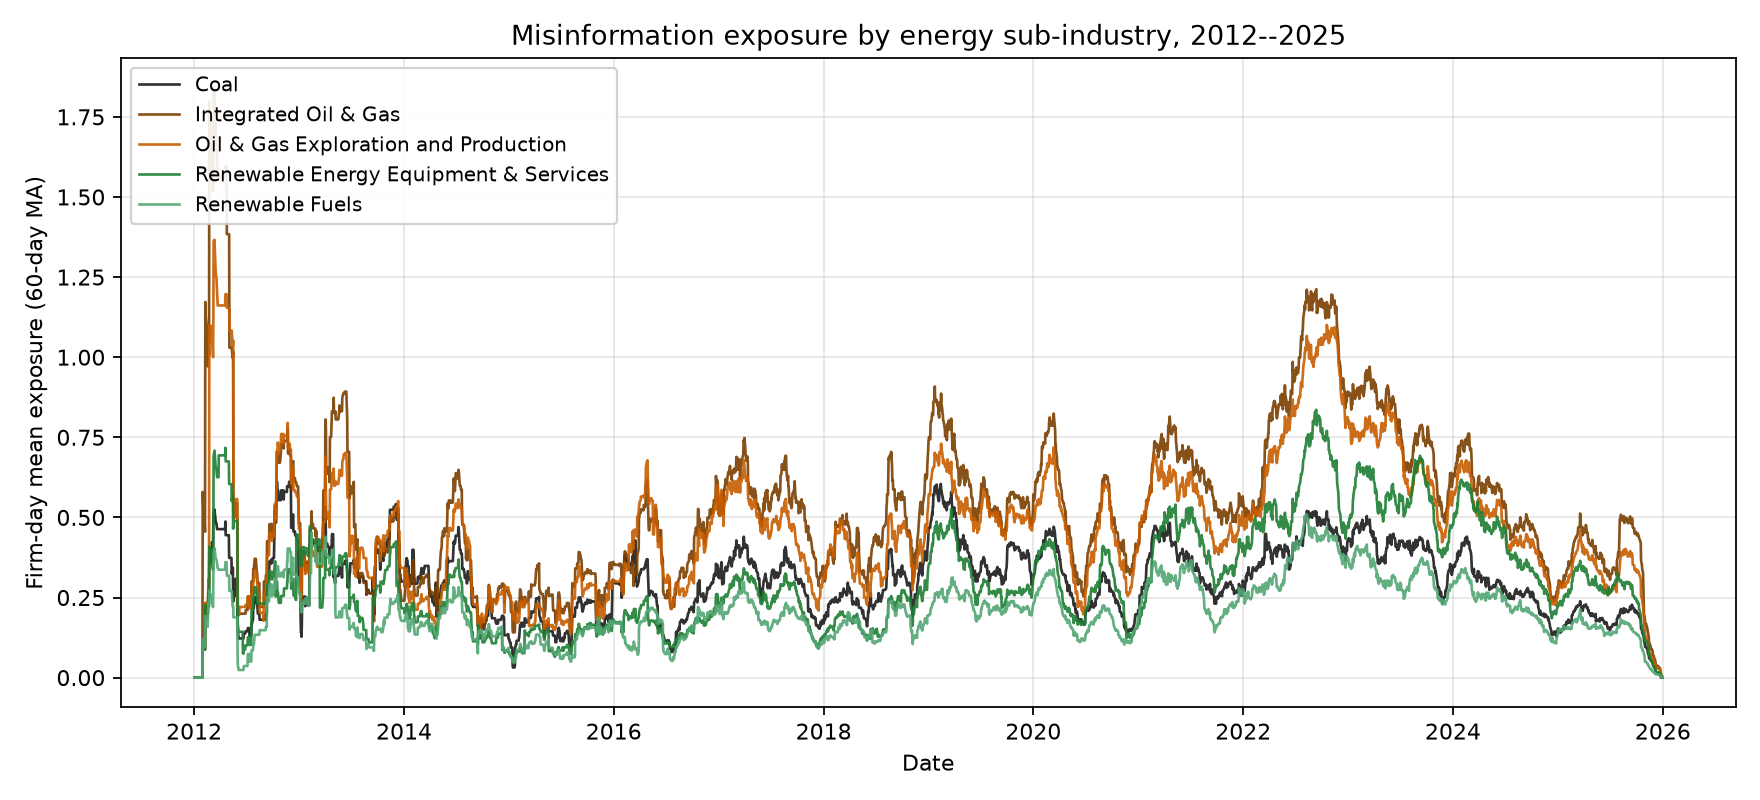
\includegraphics[width=\linewidth]{figures/fig_v2_exposure_by_industry.png}
\caption{Mean measured exposure by climate-transition sub-industry (60-day moving average). Fossil-fuel and renewable sub-industries exhibit different content patterns. This distributional contrast does not itself establish a difference in spread-response coefficients.}
\label{fig:v2_exposure_by_industry}
\end{figure}

\subsection{Model II: Misinformation and Systematic Risk (CAPM Beta)}
\label{sec:results_modelII}
The saved factor-derived diagnostic has a small, imprecise coefficient on mean exposure ($-0.0007$, security/date $p=0.53$, $N=384{,}017$). The log content-sum and misinformation-score variants are also imprecise. Table~\ref{tab:v2_full_modelII} retains the full diagnostic readout so that the risk benchmark is transparent. The input's regional factor mapping is not equivalent to actual listing markets, however, and these coefficients are not presented as validated cross-market estimates of systematic risk. A null diagnostic cannot establish that misinformation leaves correctly measured covariance risk unchanged.

\begin{table}[htbp]
\centering
\caption{Climate-Transition Panel, PanelOLS Full Readout: Model II (CAPM Beta)}
\label{tab:v2_full_modelII}
\begin{threeparttable}
\small
\setlength{\tabcolsep}{4pt}
\begin{tabular}{l r r r r r r}
\toprule
 & \multicolumn{3}{c}{$\mathrm{Exp}^{\text{mean}}$} & \multicolumn{3}{c}{$\log(1+\mathrm{Exp}^{\text{sum}})$} \\
\cmidrule(lr){2-4}\cmidrule(lr){5-7}
Term & Coef. & SE & $p$ & Coef. & SE & $p$ \\
\midrule
Exposure term & $-0.0007$ & 0.0012 & 0.525 & $-0.0002$ & 0.0005 & 0.716 \\
Log Volume & $+0.0336^{***}$ & 0.0056 & $<$0.001 & $+0.0336^{***}$ & 0.0056 & $<$0.001 \\
Log Market Cap & $-0.0398^{**}$ & 0.0200 & 0.048 & $-0.0398^{**}$ & 0.0200 & 0.048 \\
Spread Percent & $-0.0293^{**}$ & 0.0126 & 0.021 & $-0.0293^{**}$ & 0.0126 & 0.021 \\
Dividend Yield & $-0.0074^{**}$ & 0.0036 & 0.045 & $-0.0074^{**}$ & 0.0036 & 0.045 \\
Intraday Volatility & $+0.0037^{*}$ & 0.0020 & 0.072 & $+0.0037^{*}$ & 0.0020 & 0.072 \\
CPI Inflation & $-0.0217^{***}$ & 0.0065 & 0.001 & $-0.0217^{***}$ & 0.0065 & 0.001 \\
GDP Growth & $-0.0425^{***}$ & 0.0097 & $<$0.001 & $-0.0425^{***}$ & 0.0097 & $<$0.001 \\
Unemployment & $-0.0297^{***}$ & 0.0042 & $<$0.001 & $-0.0297^{***}$ & 0.0042 & $<$0.001 \\
\midrule
Observations & & & 384,017 & & & 384,017 \\
$R^2$ & & & 0.671 & & & 0.671 \\
Within $R^2$ & & & 0.052 & & & 0.052 \\
Adj.\ Within $R^2$ & & & 0.052 & & & 0.052 \\
Wald $F$ (joint) & & & 14.26 & & & 14.26 \\
Firm FE & & & Yes & & & Yes \\
Year-Month FE & & & Yes & & & Yes \\
SE clustering & & & Firm $+$ Date & & & Firm $+$ Date \\
\bottomrule
\end{tabular}
\begin{tablenotes}
\small
\item \textit{Scope:} Supplied factor-derived diagnostic. The regional factor mapping is not validated by the listing-market correction, so this table does not establish cross-market risk or return effects.\par
\item \textit{Notes:} Dependent variable: 252-day rolling CAPM beta, Equation~\ref{eq:beta_misinfo}, 204-firm climate-transition panel. The two column blocks replace the exposure
term with the firm-day mean exposure $\mathrm{Exp}^{\text{mean}}_{i,t}$ and its
concave volume variant $\log(1+\mathrm{Exp}^{\text{sum}}_{i,t})$; control
coefficients are nearly identical across the two blocks, as expected by
Frisch--Waugh--Lovell when two variants of a sparse firm-day regressor have
negligible partial correlation with the controls. Standard errors are CRV1
two-way clustered by firm (RIC) and calendar date. Continuous controls are
winsorized at the 1st and 99th percentiles; the exposure regressors are not
winsorized. $^{*}p<0.10$, $^{**}p<0.05$, $^{***}p<0.01$.
\end{tablenotes}
\end{threeparttable}
\end{table}


The distinction is consistent with the different time scales involved. A rolling 252-observation beta changes slowly, whereas the content index and quoted spreads vary daily. Volume, size, dividends, volatility and economic conditions can affect a rolling estimate in ways that differ from their association with a daily quote (\cite{StockWatson2002}; \cite{BakerBloomDavis2016}). The benchmark therefore helps define the scope of the paper: the positive evidence concerns quoted trading conditions under specified controls, rather than a general finding about changes in market risk.

\subsection{Model III: Fama--French Excess Returns}
\label{sec:results_modelIII}
The supplied excess-return diagnostic is negative for mean exposure ($-0.0224$) but loses precision when security and date are both clustered ($p=0.151$, $N=382{,}890$). Firm-only clustering produces a smaller standard error without changing the coefficient. Table~\ref{tab:v2_full_modelIII} retains this comparison. The probability-value difference illustrates why date-level dependence matters; it does not establish a return effect. The supplied regional factor and risk-free-rate mapping further limits a cross-market excess-return interpretation.

\begin{table}[htbp]
\centering
\caption{Climate-Transition Panel, PanelOLS Full Readout: Model III (Fama--French Excess Return)}
\label{tab:v2_full_modelIII}
\begin{threeparttable}
\small
\setlength{\tabcolsep}{4pt}
\begin{tabular}{l r r r r r r}
\toprule
 & \multicolumn{3}{c}{$\mathrm{Exp}^{\text{mean}}$} & \multicolumn{3}{c}{$\log(1+\mathrm{Exp}^{\text{sum}})$} \\
\cmidrule(lr){2-4}\cmidrule(lr){5-7}
Term & Coef. & SE & $p$ & Coef. & SE & $p$ \\
\midrule
Exposure term & $-0.0224$ & 0.0156 & 0.151 & $-0.0048$ & 0.0089 & 0.591 \\
FF\_MktRF & $+0.6668^{***}$ & 0.0439 & $<$0.001 & $+0.6667^{***}$ & 0.0439 & $<$0.001 \\
FF\_SMB & $+0.2003^{***}$ & 0.0450 & $<$0.001 & $+0.2002^{***}$ & 0.0450 & $<$0.001 \\
FF\_HML & $+0.4195^{***}$ & 0.0481 & $<$0.001 & $+0.4196^{***}$ & 0.0481 & $<$0.001 \\
FF\_RMW & $+0.0066$ & 0.0345 & 0.848 & $+0.0072$ & 0.0346 & 0.835 \\
FF\_CMA & $+0.0169$ & 0.0446 & 0.704 & $+0.0171$ & 0.0446 & 0.702 \\
Log Volume & $+0.1516^{***}$ & 0.0159 & $<$0.001 & $+0.1517^{***}$ & 0.0159 & $<$0.001 \\
Log Market Cap & $+0.0677^{***}$ & 0.0215 & 0.002 & $+0.0677^{***}$ & 0.0215 & 0.002 \\
Spread Percent & $+0.1435^{***}$ & 0.0279 & $<$0.001 & $+0.1434^{***}$ & 0.0279 & $<$0.001 \\
Dividend Yield & $-0.0143^{***}$ & 0.0029 & $<$0.001 & $-0.0142^{***}$ & 0.0029 & $<$0.001 \\
Intraday Volatility & $+0.0252^{**}$ & 0.0108 & 0.021 & $+0.0252^{**}$ & 0.0108 & 0.021 \\
CPI Inflation & $+0.0008$ & 0.0119 & 0.945 & $+0.0008$ & 0.0119 & 0.946 \\
GDP Growth & $+0.0077$ & 0.0173 & 0.656 & $+0.0077$ & 0.0173 & 0.658 \\
Unemployment & $-0.0068$ & 0.0081 & 0.403 & $-0.0068$ & 0.0081 & 0.400 \\
\midrule
Observations & & & 382,890 & & & 382,890 \\
$R^2$ & & & 0.077 & & & 0.077 \\
Within $R^2$ & & & 0.069 & & & 0.069 \\
Adj.\ Within $R^2$ & & & 0.069 & & & 0.069 \\
Wald $F$ (joint) & & & 36.49 & & & 36.48 \\
Firm FE & & & Yes & & & Yes \\
Year-Month FE & & & Yes & & & Yes \\
SE clustering & & & Firm $+$ Date & & & Firm $+$ Date \\
\bottomrule
\end{tabular}
\begin{tablenotes}
\small
\item \textit{Scope:} Supplied factor-derived diagnostic. The regional factor mapping is not validated by the listing-market correction, so this table does not establish cross-market risk or return effects.\par
\item \textit{Notes:} Dependent variable: daily Fama--French five-factor excess return, Equation~\ref{eq:ff5_aug}, 204-firm climate-transition panel. The two column blocks replace the exposure
term with the firm-day mean exposure $\mathrm{Exp}^{\text{mean}}_{i,t}$ and its
concave volume variant $\log(1+\mathrm{Exp}^{\text{sum}}_{i,t})$; control
coefficients are nearly identical across the two blocks, as expected by
Frisch--Waugh--Lovell when two variants of a sparse firm-day regressor have
negligible partial correlation with the controls. Standard errors are CRV1
two-way clustered by firm (RIC) and calendar date. Continuous controls are
winsorized at the 1st and 99th percentiles; the exposure regressors are not
winsorized. $^{*}p<0.10$, $^{**}p<0.05$, $^{***}p<0.01$.
\end{tablenotes}
\end{threeparttable}
\end{table}


The benchmark provides no independent return-pricing claim. More generally, a daily content coefficient added to a factor regression need not identify a priced risk factor, and an insignificant coefficient need not imply that information quality has no valuation consequences. Keeping risk, returns and quoted liquidity conceptually separate allows the positive spread association to be stated directly, while leaving the corresponding null and imprecise results visible.

\section{Discussion}
\label{sec:discussion}

The findings support a substantive connection between the climate-information environment and quoted liquidity in energy equities. In the local market-day specification, a higher sector-relevant misinformation score is associated with wider quoted spreads. This is the direction predicted when traders differ in their ability to verify climate claims and liquidity suppliers face greater information risk. The positive estimate remains after shared local trading conditions are absorbed, giving the result more substance than an uncontrolled correlation between social-media activity and financial markets. Its interpretation is an association within a specified comparison, rather than a causal cost estimate.

The theoretical contribution is to bring politically produced misinformation into a framework usually applied to the distribution of financial information. Claims about climate science, carbon restrictions, subsidies or the viability of low-carbon technologies can be costly to verify. Investors with more expertise or better access to credible information may interpret those claims differently, giving liquidity providers a reason to adjust quotes (\cite{GlostenMilgrom1985}; \cite{GrossmanStiglitz1980}; \cite{GoldsteinYang2017}). The data are consistent with that account under monthly and market-day controls. They do not observe a trader's verification decision, investor sophistication or order direction, so they do not identify that mechanism uniquely. Maintaining the distinction between a theoretical channel and its directly observed implications strengthens the contribution.

Sector-month controls locate the limit of the evidence. After those conditions are absorbed, the coefficient changes sign and is imprecise, both with contemporaneous and prior-session financial controls. This does not support a stable independent daily widening response. It also changes the economic object being estimated: shared monthly sector conditions may include genuine information-verification pressures alongside commodity-price changes, policy news and valuation uncertainty. Removing that component is a demanding local comparison, not a demonstration that the remaining coefficient alone measures the total information costs of climate misinformation. The paper therefore reports the positive broader association and the null local association together. Neither can substitute for a design that separates exogenous misinformation from the news environment in which it circulates.

The political-economy implication is most direct at the sub-industry level. Fossil-fuel chains and renewable technologies face different claims about demand, regulation and technological feasibility. A coal-security trader and a renewable-fuels trader can therefore face different relevant narratives on the same date. The sector-sensitive measure represents that distinction rather than assigning every security the same daily content value. The observed fossil--renewable exposure divergence is informative about the distribution of contested content, even though the formal post-2019 interaction does not establish a stronger liquidity response. This is a measurement contribution with substantive content, rather than merely a choice of regression fixed effects.

The wider literature gives that distinction practical significance. Misinformation can affect beliefs, trust and collective action, while energy investment depends on expectations about policy and technology (\cite{cobb2025politics}; \cite{farrell2016network}; \cite{engle2020hedging}; \cite{bolton2021climate}). A liquid secondary market can matter to financial conditions surrounding the transition, but this paper does not observe the cost of financing a new project or an issuer's investment decision. The evidence speaks to posted trading terms in listed equities. Connecting those terms to primary financing or real investment would require additional data and an identified transmission mechanism. The market-liquidity contribution is useful on its own without making that additional claim.

The corpus also highlights why the supply of misinformation and its audience should be kept distinct. The reach-based arguments of \textcite{acemoglu2010spread} and \textcite{VosoughiRoyAral2018} motivate attention to diffusion, but the daily index averages classified content without weighting it by observed investor exposure. The supplied engagement and owner-network summaries document a heavy-tailed public information environment; they do not show which investors saw a post. Likewise, volume and relevance variants do not establish a positive coefficient in the fully conditional model. The appropriate interpretation is that sector-sensitive content captures a plausible information environment whose financial association depends on the comparison, not that a high post score constitutes a measured dose of investor misinformation.

Three limitations remain particularly relevant. First, the English-language, keyword-selected corpus has uneven geographic and temporal coverage. This matters in markets such as mainland China and Indonesia, which account for many sample securities, and cannot be solved by relabelling the content as globally representative. Second, rubric-development checks helped define the classifier but do not supply independent precision, recall or human agreement. The content measure is reproducible from persisted scores, while its external accuracy remains a separate empirical question (\cite{grimmer2022text}; \cite{gilardi2023chatgpt}). Third, nine sector-level information series limit cluster-based inference despite the large number of security-day rows. The alternative covariance and leave-out checks describe that uncertainty transparently instead of treating sample size as independent information.

For research on the political economy of climate finance, these results provide a clear basis for further work. Sector-specific classification retains the political and economic content needed for a meaningful market comparison. Correctly assigned market-day effects establish that the positive association is not simply a common local-market movement. Sector-month controls then show that the evidence does not isolate an additional daily misinformation response. Those are complementary findings. An event study or instrument grounded in a defensible information shock, together with local-close timestamps and direct investor-flow data, would be needed to distinguish persistent information conditions from a causal trading-cost effect.

\section{Conclusions}
\label{sec:conclusion}

Climate misinformation is associated with wider quoted spreads in the monthly and local market-day specifications for climate-transition equities. The positive local market-day estimate establishes a connection between sector-relevant climate content and trading conditions after shared local daily shocks are absorbed. The finding is consistent with information-verification costs and supports bringing the political production of climate misinformation into research on market liquidity. Its empirical boundary is equally clear: adding sector-month controls changes the sign and leaves an imprecise coefficient, including in the model with prior-session financial controls.

Four conclusions follow. First, the construction of the content measure matters. Classifying posts separately against nine energy sub-industries preserves differences in the political information relevant to fossil-fuel and renewable securities. The resulting within-date variation makes a local market-day comparison possible. It does not create independent treatment at the level of each security, and inference must respect the sector assignment.

Second, the positive spread association is conditional on the sector comparison. It is statistically discernible under local market-day effects but does not persist as a robust positive coefficient after sector-month conditions are removed. The evidence therefore supports an association in the broader sector information environment while leaving a distinct daily causal response unresolved. The null result narrows the claim without requiring that climate misinformation be considered economically unimportant.

Third, the complementary VWAP-gap and timing checks provide no separate robust response under the fully conditional design. The gap is not per-dollar transaction price impact, and a lag is not an exogenous information shock. The risk and excess-return diagnostics are also inconclusive and constrained by their supplied factor mapping. They are retained as boundaries on the financial interpretation rather than used to amplify the main result.

Fourth, the corpus and sub-industry profiles document an uneven climate-information environment. The increase in content volume after 2019 and the fossil--renewable exposure divergence motivate sector-sensitive measurement, but the formal slope interaction does not establish a strengthened spread relationship. This distinction keeps a substantive distributional finding separate from a claim about changing financial sensitivity.

The paper contributes a sector-sensitive bridge between the political production of climate misinformation and the quoted trading environment of energy equities. Future work can build on that bridge through independent multilingual validation, exchange-local information timing, defensible exogenous events and direct measures of investor participation. Applying the same construction to other domains of politically contested knowledge---public health, technology and financial regulation---would also test how broadly the relationship extends (\cite{lins2017social}; \cite{taber2006motivated}). The present evidence establishes where the positive liquidity association is observed and states clearly where the data do not support a stronger claim.

\section*{Ethics and data availability}
The source research received institutional ethics approval for the Meta Content Library analysis. The replication materials supply the financial analysis, fixed classifications, saved estimates, source tables and figure assets. Raw Meta Content Library records and post text are access-controlled; financial observations originate from licensed Refinitiv data. The financial robustness tables reproduce from the documented fixed inputs. Reconstructing the supplied corpus engagement summaries and owner-network figures requires authorized platform records. An author-identified repository link is supplied with the title page.
\section*{Declaration of generative AI and AI-assisted technologies}
OpenAI Codex (GPT-6) assisted with analysis-code development, reproducible visualization and targeted manuscript editing. Numerical estimates are generated by the documented statistical computations from fixed inputs. Language-model classification is described as a research method in Section~\ref{sec:LLM}. Scientific interpretation, verification and submission remain the author's responsibility.

\printbibliography

\appendix
\section*{Appendix}
Section~\ref{sec:appendix_financial} reports descriptive statistics for the financial panel (Tables~\ref{tab:panel_a}--\ref{tab:panel_f}), and Section~\ref{sec:appendix_climate} reports coverage and composition for the climate-transition equity panel. Section~\ref{sec:appendix_corpus} documents the misinformation corpus (Tables~\ref{tab:panel_g}--\ref{tab:panel_n}), including misinformation type and reach in Section~\ref{sec:firmday_corpus_intuition}. Section~\ref{sec:appendix_network} maps the dissemination network, Section~\ref{sec:firmday_validation} describes the exposure index and rubric-development checks, and Section~\ref{sec:appendix_heterogeneity} reports the heterogeneity and interaction checks.

\section{Financial Panel Descriptive Statistics}
\label{sec:appendix_financial}

The merged firm-level panel comprises 19,183,738 firm-day observations across 5,375 unique equity securities spanning 2012--2025. Table~\ref{tab:panel_a} reports summary statistics - including observation counts, fill rates, means, standard deviations, and full distributional percentiles - for nine firm-level trading variables (prices, volume, market capitalization, dividend yield, bid-ask spreads, returns, and CAPM beta), three macroeconomic controls (GDP growth, unemployment, CPI inflation), and the five Fama-French factors (MktRF, SMB, HML, RMW, CMA). The table is presented in landscape orientation to accommodate the eleven-column layout.

\begin{sidewaystable}[htbp]
\centering
\footnotesize
\setlength{\tabcolsep}{3.5pt}
\begin{tabular}{l l r r r r r r r r r}
\toprule
\textbf{Variable} & \textbf{Unit} & \textbf{N} & \textbf{Fill\%} & \textbf{Mean} & \textbf{SD} & \textbf{Min} & \textbf{P25} & \textbf{Median} & \textbf{P75} & \textbf{Max} \\
\midrule
\multicolumn{11}{l}{\textit{Firm-Level Variables}} \\
  Price Close & source currency & 13,759,934 & 71.7 & 388.67 & 2,128.98 & 0.01 & 10.96 & 30.58 & 118.26 & 359,900.00 \\
  Volume & shares & 18,394,237 & 95.9 & 9.03M & 60.58M & 0.00 & 0.00 & 0.823M & 5.08M & 45,941.76M \\
  Company Market Cap & source currency & 14,263,811 & 74.4 & 1,860,901.54 & 21,101,237.64 & 14.87 & 5,032.21 & 15,080.74 & 104,672.42 & 2,464,175,093.59 \\
  Dividend yield & \% & 12,626,836 & 65.8 & 2.38 & 8.49 & 0.00 & 0.48 & 1.72 & 3.49 & 20,316.87 \\
  BidAskSpread & source currency & 13,419,146 & 70.0 & 4.24 & 61.02 & -268.00 & 0.01 & 0.04 & 0.30 & 13,550.00 \\
  SpreadPercent & \% & 13,419,145 & 70.0 & 0.54 & 1.95 & -200.00 & 0.07 & 0.16 & 0.37 & 172.14 \\
  DailyReturn &  & 13,255,243 & 69.1 & 0.09 & 115.33 & -73.29 & -1.04 & 0.00 & 1.01 & 419,653.09 \\
  CAPM\_Beta &  & 13,802,427 & 71.9 & 0.54 & 0.48 & -11.74 & 0.22 & 0.47 & 0.82 & 298.91 \\
  TotalReturn &  & 13,735,222 & 71.6 & 0.10 & 113.30 & -98.58 & -1.04 & 0.00 & 1.02 & 419,653.09 \\
\midrule
\multicolumn{11}{l}{\textit{Macroeconomic Controls}} \\
  GDP Growth & \% & 19,183,738 & 100.0 & 3.55 & 2.90 & -10.05 & 1.82 & 2.79 & 6.07 & 8.57 \\
  Stored unemployment series & \% & 19,183,738 & 100.0 & 74.87 & 12.97 & 53.10 & 63.52 & 80.07 & 82.02 & 92.19 \\
  CPI Inflation & \% & 19,183,738 & 100.0 & 1.89 & 1.52 & -0.23 & 0.98 & 1.92 & 2.62 & 8.83 \\
\midrule
\multicolumn{11}{l}{\textit{Fama--French Five Factors}} \\
  FF MktRF & \% & 18,987,538 & 99.0 & 0.03 & 1.01 & -12.01 & -0.44 & 0.05 & 0.55 & 10.03 \\
  FF SMB & \% & 18,987,538 & 99.0 & -0.01 & 0.53 & -4.81 & -0.30 & 0.00 & 0.29 & 5.71 \\
  FF HML & \% & 18,987,538 & 99.0 & 0.01 & 0.66 & -5.03 & -0.32 & 0.00 & 0.33 & 6.73 \\
  FF RMW & \% & 18,987,538 & 99.0 & 0.01 & 0.43 & -3.76 & -0.23 & 0.00 & 0.25 & 4.25 \\
  FF CMA & \% & 18,987,538 & 99.0 & 0.00 & 0.40 & -2.92 & -0.21 & 0.00 & 0.21 & 2.47 \\
\bottomrule
\end{tabular}
\caption{Panel~A: Summary statistics for key variables in the merged dataset. The sample spans 2012--2025 and covers 5,375 RICs. Fill\% indicates the proportion of non-missing observations for each variable. All firm-level variables are at daily frequency.}
\label{tab:panel_a}
\end{sidewaystable}

The supplied equity assembly uses five stored region groups. These are input labels, not a validated listing-market classification; the spread analysis uses the exchange-based crosswalk instead. Table~\ref{tab:panel_b} reports the number of firm-day observations and unique RICs per region, alongside fill rates for closing prices, CAPM beta, and Fama-French factors. The stored CN group contributes 41.2\% of input observations, the US group 31.7\% and the JP group 23.8\%; UK and EU groups account for the remainder. These percentages describe the supplied grouping, not corrected listing-market shares.

\begin{table}[!ht]
\centering
\footnotesize
\begin{tabular}{l r r r r r r r r}
\toprule
\textbf{Region} & \textbf{Obs} & \textbf{Share\%} & \textbf{RICs} & \textbf{First} & \textbf{Last} & \textbf{Price\%} & \textbf{Beta\%} & \textbf{FF\%} \\
\midrule
  CN & 7,897,640 & 41.2 & 2,231 & 2012-01-02 & 2025-12-31 & 62.3 & 63.0 & 100.0 \\
  US & 6,075,274 & 31.7 & 1,712 & 2012-01-02 & 2025-12-31 & 71.6 & 69.7 & 97.0 \\
  JP & 4,558,053 & 23.8 & 1,253 & 2012-01-02 & 2025-12-31 & 85.2 & 87.4 & 99.7 \\
  UK & 364,446 & 1.9 & 100 & 2012-01-02 & 2025-12-31 & 93.4 & 92.7 & 100.0 \\
  EU & 288,325 & 1.5 & 79 & 2012-01-02 & 2025-12-31 & 94.2 & 92.8 & 100.0 \\
\midrule
  \textbf{Total} & \textbf{19,183,738} & 100.0 & \textbf{5,375} & & & & & \\
\bottomrule
\end{tabular}
\caption{Panel~B: Coverage by stored region group. Share\% is the fraction of total firm-day observations. Price\%, Beta\%, and FF\% indicate the fill rate for Price Close, CAPM Beta, and Fama--French factors, respectively.}
\label{tab:panel_b}
\end{table}

Temporal stability is a desirable property for panel econometric analysis, as changing panel composition can introduce survivorship bias. Table~\ref{tab:panel_c} reports annual observation counts, the number of distinct securities, and non-missing rates for key variables across all fourteen sample years. The constant RIC count of 5,375 per year describes the supplied calendar grid, rather than demonstrating a survivor-bias-free investment universe, while data fill rates for prices, returns, and betas increase monotonically over time as coverage improves.

\begin{table}[!ht]
\centering
\footnotesize
\begin{tabular}{r r r r r r}
\toprule
\textbf{Year} & \textbf{Obs} & \textbf{RICs} & \textbf{Price\%} & \textbf{Return\%} & \textbf{Beta\%} \\
\midrule
  2012 & 1,363,092 & 5,375 & 53.6 & 51.3 & 25.2 \\
  2013 & 1,356,566 & 5,375 & 54.7 & 52.2 & 57.3 \\
  2014 & 1,366,584 & 5,375 & 55.8 & 53.3 & 58.0 \\
  2015 & 1,365,143 & 5,375 & 56.9 & 54.4 & 59.4 \\
  2016 & 1,367,945 & 5,375 & 59.3 & 56.5 & 61.2 \\
  2017 & 1,360,941 & 5,375 & 64.4 & 61.8 & 64.9 \\
  2018 & 1,368,416 & 5,375 & 68.1 & 65.4 & 70.3 \\
  2019 & 1,373,060 & 5,375 & 71.3 & 68.5 & 73.4 \\
  2020 & 1,376,595 & 5,375 & 75.4 & 72.7 & 76.8 \\
  2021 & 1,377,392 & 5,375 & 82.4 & 80.0 & 83.1 \\
  2022 & 1,373,896 & 5,375 & 87.2 & 84.6 & 89.3 \\
  2023 & 1,372,026 & 5,375 & 90.1 & 87.4 & 93.1 \\
  2024 & 1,382,316 & 5,375 & 91.8 & 88.8 & 96.5 \\
  2025 & 1,379,766 & 5,375 & 92.4 & 89.6 & 97.7 \\
\bottomrule
\end{tabular}
\caption{Panel~C: Annual coverage. Obs is the number of firm-day observations per year; RICs is the number of distinct securities observed that year. Price\%, Return\%, and Beta\% are non-missing rates for Price Close, DailyReturn, and CAPM Beta.}
\label{tab:panel_c}
\end{table}

Before estimating the main regression specifications, it is useful to examine the bivariate relationships among key continuous variables for evidence of multicollinearity or unexpected sign patterns. Table~\ref{tab:panel_d} presents the upper-triangle pairwise correlation matrix for daily returns, CAPM beta, percentage bid--ask spread, volume, market capitalization, and the three primary Fama-French factors. Correlations are generally modest in magnitude, with the largest off-diagonal entries appearing between MktRF and SMB ($r = -0.14$) and between MktRF and HML ($r = -0.15$).

\begin{table}[!ht]
\centering
\footnotesize
\setlength{\tabcolsep}{4pt}
\begin{tabular}{lrrrrrrrr}
\toprule
 & \textbf{Return} & \textbf{Beta} & \textbf{Spread\%} & \textbf{Volume} & \textbf{MktCap} & \textbf{MktRF} & \textbf{SMB} & \textbf{HML} \\
\midrule
  Return & 1.00 & 0.17 & 0.02 & 0.00 & 0.03 & 0.00 & -0.00 & -0.00 \\
  Beta &  & 1.00 & -0.23 & -0.01 & -0.05 & -0.00 & -0.00 & -0.00 \\
  Spread\% &  &  & 1.00 & -0.02 & 0.01 & 0.00 & -0.00 & -0.01 \\
  Volume &  &  &  & 1.00 & 0.07 & -0.00 & 0.00 & 0.00 \\
  MktCap &  &  &  &  & 1.00 & 0.00 & -0.00 & -0.00 \\
  MktRF &  &  &  &  &  & 1.00 & -0.14 & -0.15 \\
  SMB &  &  &  &  &  &  & 1.00 & 0.05 \\
  HML &  &  &  &  &  &  &  & 1.00 \\
\bottomrule
\end{tabular}
\caption{Panel~D: Pairwise correlations among key variables. Empty cells below the diagonal are suppressed for readability.}
\label{tab:panel_d}
\end{table}

Fama-French factor returns are matched to each firm based on its listing region, with four regional factor sets covering Asia Pacific, the United States, Japan, and Europe. Table~\ref{tab:panel_e} reports the number of matched observations, fill rates, and mean daily values for all five factors by region. The US market excess return exhibits the highest mean (0.056\% per day), while Japan exhibits the largest standard deviation (1.153\%).

\begin{table}[!ht]
\centering
\footnotesize
\begin{tabular}{l r r r r r r r r}
\toprule
\textbf{FF Region} & \textbf{Obs} & \textbf{Fill\%} & \textbf{MktRF} & \textbf{SD(MktRF)} & \textbf{SMB} & \textbf{HML} & \textbf{RMW} & \textbf{CMA} \\
\midrule
  AsiaPac & 7,897,640 & 100.0 & 0.019 & 0.856 & -0.007 & 0.021 & 0.018 & 0.006 \\
  US & 6,075,274 & 97.0 & 0.056 & 1.084 & -0.009 & -0.003 & 0.006 & -0.003 \\
  Japan & 4,558,053 & 99.7 & 0.033 & 1.153 & 0.002 & 0.012 & 0.000 & 0.005 \\
  Europe & 652,771 & 100.0 & 0.033 & 1.028 & 0.000 & 0.009 & 0.006 & 0.001 \\
\bottomrule
\end{tabular}
\caption{Panel~E: Fama-French five-factor summary by region mapping. Mean daily factor returns are reported. Fill\% indicates the proportion of firm-day observations matched to factors.}
\label{tab:panel_e}
\end{table}

The microstructure variables reported in Table~\ref{tab:panel_f} include the percent quoted spread used as the primary liquidity outcome and supplied daily price-gap fields. The table documents observation counts, the number of securities with non-missing data, and distributional summaries for eight trade-level variables: bid--ask spread, percentage spread, order flow, trade intensity, supplied buyer/seller indicators, volume-weighted average price (VWAP), and the absolute VWAP--midpoint percentage gap. Source field names do not identify signed order-flow quantities or per-dollar transaction impact. Coverage is near-universal for spread and order-flow variables (5,343 of 5,375 RICs) but lower for trade intensity (2,029 RICs), reflecting cross-exchange differences in tick-level data availability.

\begin{table}[!ht]
\centering
\footnotesize
\begin{tabular}{l r r r r r}
\toprule
\textbf{Variable} & \textbf{N} & \textbf{RICs} & \textbf{Mean} & \textbf{SD} & \textbf{Median} \\
\midrule
  BidAskSpread & 13,419,146 & 5,343 & 4.24 & 61.02 & 0.04 \\
  SpreadPercent & 13,419,145 & 5,343 & 0.54 & 1.95 & 0.16 \\
  OrderFlow & 13,268,923 & 5,343 & 0.08 & 193.08 & 0.00 \\
  TradeIntensity & 5,146,749 & 2,029 & 4,750.04 & 12,478.89 & 2,198.00 \\
  BuyerInitiated & 13,837,387 & 5,343 & 0.48 & 0.50 & 0.00 \\
  SellerInitiated & 13,837,387 & 5,343 & 0.47 & 0.50 & 0.00 \\
  VWAP & 13,584,674 & 5,343 & 392.92 & 2,115.66 & 30.53 \\
  PriceImpact & 13,268,922 & 5,343 & 0.68 & 47.95 & 0.37 \\
\bottomrule
\end{tabular}
\caption{Panel~F: Microstructure-variable coverage. The percent quoted spread is the main liquidity outcome. PriceImpact is a supplied field name for the absolute VWAP--midpoint percentage gap, not transaction price impact. N is the number of non-missing observations; RICs is the number of distinct securities with at least one non-missing value.}
\label{tab:panel_f}
\end{table}

\begin{table}[htbp]
\centering
\caption{Mean CAPM Beta by Region and Market-Capitalisation Quintile}
\label{tab:beta_region_mktcap}
\begin{threeparttable}
\small
\begin{tabular}{l r r r r r r}
\toprule
Region & Mean $\beta$ & Median $\beta$ & Q1 (Small) & Q2 & Q3 & Q5 (Large) \\
\midrule
CN & 0.655 & 0.594 & 0.643 & 0.673 & 0.667 & 0.600 \\
US & 0.488 & 0.388 & 0.806 & 0.837 & 0.823 & 0.166 \\
JP & 0.415 & 0.330 & 0.263 & 0.283 & 0.303 & 0.825 \\
UK & 0.747 & 0.714 & 0.731 & 0.785 & 0.782 & 0.570 \\
EU & 0.905 & 0.877 & 0.816 & 0.967 & 0.897 & 0.995 \\
\bottomrule
\end{tabular}
\begin{tablenotes}\small
\item \textit{Notes:} Mean rolling CAPM beta computed from 252-day OLS windows requiring minimum 126 observations. Quintiles defined by Company Market Cap within each region-day. The low overall mean (0.54) is driven by Japanese firms (0.42) and the preponderance of small-cap US firms in the sample. Non-synchronous trading bias (\cite{ScholesWilliams1977}) likely contributes to downward bias in thinly traded securities.
\end{tablenotes}
\end{threeparttable}
\end{table}

\FloatBarrier
\section{Climate-Transition Panel Descriptive Statistics}
\label{sec:appendix_climate}

This subsection reports descriptive statistics for the unique climate-transition firm panel used in the subsample regressions. The objective is to document coverage, composition, and distributional properties before estimation. Across all three tables below, the sample is defined by renewable and fossil-fuel TRBC mappings with utilities excluded, consistent with the main-text climate-transition specifications.

\begin{table}[htbp]
\centering
\caption{Climate-Transition Panel Coverage Summary}
\label{tab:energy_desc_coverage}
\begin{threeparttable}
\small
\begin{tabular}{l r}
\toprule
Metric & Value \\
\midrule
Firm-day observations & 726,890 \\
Unique securities (RICs) & 204 \\
Start date & 2012-01-02 \\
End date & 2025-12-31 \\
Unique year-month bins & 168 \\
Median observations per firm & 3,588 \\
\bottomrule
\end{tabular}
\begin{tablenotes}\small
\item \textit{Notes:} Coverage statistics for the full financial input, before the content-window, quote, trading and complete-case filters. These are not regression sample sizes.
\end{tablenotes}
\end{threeparttable}
\end{table}

\begin{table}[htbp]
\centering
\caption{Climate-Transition Panel Composition by Stored Region Group (Unique Securities)}
\label{tab:energy_desc_region}
\begin{threeparttable}
\small
\begin{tabular}{l r r}
\toprule
Region & Unique securities & Share (\%) \\
\midrule
US & 102 & 50.00 \\
CN & 83 & 40.69 \\
JP & 15 & 7.35 \\
EU & 2 & 0.98 \\
UK & 2 & 0.98 \\
\bottomrule
\end{tabular}
\begin{tablenotes}\small
\item \textit{Notes:} Shares describe the supplied region groups for 204 securities, not actual listing markets. The market crosswalk and corrected market composition are reported separately.
\end{tablenotes}
\end{threeparttable}
\end{table}

\begin{table}[htbp]
\centering
\caption{Climate-Transition Panel Key Variable Descriptive Statistics}
\label{tab:energy_desc_vars}
\begin{threeparttable}
\small
\setlength{\tabcolsep}{4pt}
\begin{tabular}{l r r r r r r}
\toprule
Variable & N & Mean & Std. Dev. & P25 & Median & P75 \\
\midrule
SpreadPercent & 504,043 & 0.6147 & 1.6705 & 0.0607 & 0.1590 & 0.4090 \\
CAPM\_Beta & 525,697 & 0.5679 & 0.4984 & 0.2039 & 0.5168 & 0.8864 \\
ExcessReturn & 506,612 & 0.0328 & 2.6949 & -1.2207 & -0.0100 & 1.1272 \\
log\_volume & 698,179 & 11.3694 & 6.8472 & 5.7071 & 14.5147 & 16.3631 \\
log\_mktcap & 559,387 & 25.0607 & 2.7631 & 22.9046 & 24.3402 & 27.1216 \\
IntradayVolatility & 496,614 & 3.4611 & 2.5748 & 1.7758 & 2.7528 & 4.3222 \\
DivYield & 464,457 & 2.9153 & 3.6049 & 0.2509 & 1.8536 & 4.1325 \\
cpi\_inflation & 726,890 & 2.1371 & 1.5976 & 1.2616 & 2.0000 & 2.6195 \\
gdp\_growth & 726,890 & 3.8414 & 2.6520 & 2.3402 & 2.8876 & 6.0685 \\
unemployment (stored) & 726,890 & 73.1123 & 11.1097 & 63.5234 & 80.0325 & 80.4977 \\
\bottomrule
\end{tabular}
\begin{tablenotes}\small
\item \textit{Notes:} Statistics correspond to the estimation sample after standard preprocessing used in the econometric pipeline (including transformations and winsorisation for relevant continuous variables).
\end{tablenotes}
\end{threeparttable}
\end{table}

The descriptive profile in Tables~\ref{tab:energy_desc_coverage}--\ref{tab:energy_desc_vars} motivates the energy-subsample strategy. The panel is sufficiently long and dense for two-way FE estimation, yet actual listing composition is concentrated in mainland China and Indonesia, making local market-day effects and inference at the sector assignment level important.

\FloatBarrier
\FloatBarrier
\begin{table}[htbp]
\centering
\caption{Listing-market composition of the principal sample}
\label{tab:markets}
\begin{minipage}{\linewidth}
\small
\setlength{\tabcolsep}{4pt}
\begingroup\centering
\begin{tabular}{p{0.43\linewidth}rrr}
\toprule
Listing market & Securities & Security-days & Mean spread \\
\midrule
Brazil & 8 & 18,945 & 0.256 \\
France & 1 & 3,519 & 0.038 \\
Germany & 1 & 1,286 & 0.085 \\
Hong Kong & 5 & 16,465 & 0.226 \\
Indonesia & 62 & 111,633 & 1.756 \\
Japan & 3 & 10,104 & 0.172 \\
Mainland China & 82 & 197,427 & 0.157 \\
Malaysia & 1 & 3,373 & 0.505 \\
Netherlands & 1 & 3,516 & 0.042 \\
Taiwan & 12 & 32,073 & 0.622 \\
United Kingdom & 2 & 6,962 & 0.028 \\
United States & 24 & 80,497 & 0.070 \\
\bottomrule
\end{tabular}\par\endgroup
\par\vspace{0.5em}\footnotesize Market comes from the listing-exchange suffix. Mean spreads are raw percentages before tail capping. Market-day effects absorb all observed local securities together; counts do not measure independent shocks.
\end{minipage}
\end{table}

\begin{table}[htbp]
\centering
\caption{Estimation sample construction}
\label{tab:flow}
\begin{minipage}{\linewidth}
\small
\setlength{\tabcolsep}{4pt}
\begingroup\centering
\begin{tabular}{p{0.72\linewidth}r}
\toprule
Filter & Security-days \\
\midrule
Financial input & 726,890 \\
Within content window & 715,200 \\
Positive valid quotes and active trading & 489,929 \\
Contemporaneous-control complete cases & 486,655 \\
Prior-session-control complete cases & 485,800 \\
\bottomrule
\end{tabular}\par\endgroup
\par\vspace{0.5em}\footnotesize The two complete-case rows are alternative control choices applied to the same eligible quote sample, not sequential filters. Content window is 3 January 2012 to 13 October 2025. Active trading requires positive volume and a positive close.
\end{minipage}
\end{table}

\FloatBarrier
\section{Descriptive Statistics and Supporting Tables}
\label{sec:appendix_corpus}

The corpus comprises 265,652 public Facebook posts with platform-reported engagement data. Table~\ref{tab:panel_g} provides distributional summaries for all engagement metrics - likes, shares, comments, total reactions (including emoji-specific breakdowns for angry, love, haha, sad, wow, and care reactions), and view counts - as well as text-level characteristics (character length and word count). The large gap between mean and median values for most engagement variables reflects the heavy right skew characteristic of social media diffusion, where a small number of viral posts account for a disproportionate share of total engagement.

\begin{table}[!ht]
\centering
\caption{Social Media Post Summary Statistics}
\label{tab:panel_g}
\begin{threeparttable}
\begin{tabularx}{\textwidth}{l R R R R R R}
\toprule
Variable & N & Mean & Median & Std.Dev. & Min & Max \\
\midrule
Likes & 262,461 & 140.8 & 10.00 & 2,015.6 & 0.000 & 525,472.0 \\
Shares & 265,651 & 44.90 & 2.00 & 682.3 & 0.000 & 81,948.0 \\
Comments & 265,651 & 22.72 & 0.000 & 217.6 & 0.000 & 39,790.0 \\
Total Reactions & 262,492 & 175.9 & 13.00 & 2,278.2 & 0.000 & 531,508.0 \\
Views & 220,511 & 10,372.8 & 1,625.0 & 91,127.8 & 101.0 & 15,900,642 \\
Angry Reactions & 262,461 & 7.69 & 0.000 & 225.5 & 0.000 & 57,470.0 \\
Love Reactions & 262,461 & 15.38 & 0.000 & 267.5 & 0.000 & 46,490.0 \\
Haha Reactions & 262,461 & 3.84 & 0.000 & 89.18 & 0.000 & 31,575.0 \\
Sad Reactions & 262,461 & 3.52 & 0.000 & 162.2 & 0.000 & 44,420.0 \\
Wow Reactions & 262,461 & 1.66 & 0.000 & 31.79 & 0.000 & 7,074.0 \\
Care Reactions & 262,461 & 0.000 & 0.000 & 0.000 & 0.000 & 0.000 \\
Text Length (chars) & 265,652 & 3,599.1 & 1,337.0 & 6,828.6 & 2.00 & 168,477.0 \\
Word Count & 265,652 & 553.9 & 197.0 & 1,062.6 & 1.00 & 26,148.0 \\
\bottomrule
\end{tabularx}
\begin{tablenotes}\small
\item \textit{Notes:} Summary statistics for 265,652 social media posts from the Meta Content Library (MCL). Engagement metrics reflect platform-reported counts at the time of data collection.
\end{tablenotes}
\end{threeparttable}
\end{table}

The 217,954 unique posts paired by calendar date to the climate-transition panel span 2012 through 2025. Table~\ref{tab:panel_j} reports their annual distribution, with the misinformation classification produced by the Qwen3.6-35B-A3B model (Section~\ref{sec:LLM}): a post is counted as misinformation if its continuous misinformation score reaches the rubric's ``clearly false or pseudoscientific climate/energy claims'' threshold of 50 on the 0--100 scale. Post volume rises sharply after 2019, coinciding with the intensification of global climate activism and the digital migration associated with the COVID-19 pandemic, while Qwen-classified misinformation prevalence fluctuates between 1.7\% and 5.0\% across years. The within-year movement is not proportional to raw post volume: prevalence peaks in the contested-policy years 2012 (5.0\%), 2017 (3.0\%), 2019 (3.2\%), and 2022 (3.0\%), and falls to its sample minimum in the highest-volume years 2024--2025 ($\approx$1.7\%), where general climate content grows faster than misinformation.

\begin{table}[!ht]
\centering
\caption{Annual Distribution of Posts and Qwen-Classified Misinformation Prevalence}
\label{tab:panel_j}
\begin{threeparttable}
\begin{tabularx}{\textwidth}{l R R R R R}
\toprule
Year & Total Posts & Misinfo.\ Posts & Prevalence (\%) & Mean Likes & Mean Shares \\
\midrule
2012 & 1,276 & 64 & 5.02 & 86.2 & 38.96 \\
2013 & 2,649 & 82 & 3.10 & 87.5 & 39.97 \\
2014 & 3,885 & 88 & 2.27 & 87.8 & 33.56 \\
2015 & 5,106 & 95 & 1.86 & 115.5 & 47.93 \\
2016 & 9,954 & 272 & 2.73 & 138.2 & 82.97 \\
2017 & 13,845 & 413 & 2.98 & 93.7 & 58.13 \\
2018 & 11,429 & 268 & 2.34 & 66.2 & 45.01 \\
2019 & 17,160 & 542 & 3.16 & 90.6 & 47.83 \\
2020 & 17,118 & 427 & 2.49 & 128.0 & 61.19 \\
2021 & 23,038 & 469 & 2.04 & 112.9 & 38.67 \\
2022 & 24,102 & 710 & 2.95 & 86.9 & 22.68 \\
2023 & 25,846 & 731 & 2.83 & 76.7 & 21.54 \\
2024 & 30,404 & 538 & 1.77 & 88.3 & 26.95 \\
2025 & 32,142 & 552 & 1.72 & 344.6 & 62.91 \\
\midrule
Total & 217,954 & 5,251 & 2.41 & 132.4 & 43.03 \\
\bottomrule
\end{tabularx}
\begin{tablenotes}\small
\item \textit{Notes:} Annual counts for the 217,954 unique posts paired by date to the climate-transition panel. ``Misinfo.\ Posts'' counts posts whose Qwen3.6-35B-A3B misinformation score reaches the threshold of 50; ``Prevalence'' is that count as a share of the year's posts.
\end{tablenotes}
\end{threeparttable}
\end{table}

The Meta Content Library organizes posts into eight keyword-based thematic datasets covering different dimensions of climate discourse. Table~\ref{tab:panel_k} breaks down post coverage, Qwen-classified misinformation counts, engagement, and unique owner counts by source dataset. The pattern is intuitive given how the model reasons about content: the explicitly political ``combined'' multi-keyword set (6.4\% prevalence) and the climate-politics set (1.9\%) concentrate the misinformation, because that is where contested claims about climate science and policy are made, whereas the adaptation, resilience, and ecological datasets---which collect operational and scientific content---sit at or below 0.2\% prevalence. The classifier is not flagging climate \emph{topicality}; it is flagging the false or misleading \emph{claims} that cluster in the political corners of the corpus.

\begin{table}[!ht]
\centering
\caption{Post Coverage by MCL Source Dataset (Qwen-Classified Misinformation)}
\label{tab:panel_k}
\begin{threeparttable}
\begin{tabularx}{\textwidth}{l R R R R R R}
\toprule
Source Dataset & Posts & Misinfo. & Prev.\ (\%) & Mean Likes & Mean Shares & Owners \\
\midrule
Combined & 65,688 & 4,180 & 6.4 & 144.8 & 69.73 & 25,171 \\
Climate Change Adaptation Al.. & 61,079 & 126 & 0.2 & 48.10 & 11.12 & 17,931 \\
Climate Change Politics All .. & 32,930 & 618 & 1.9 & 153.2 & 69.05 & 14,527 \\
Climate Change Global Justic.. & 14,406 & 134 & 0.9 & 120.4 & 38.57 & 7,369 \\
Climate Change Global Resili.. & 13,448 & 18 & 0.1 & 68.60 & 11.55 & 7,019 \\
Climate Change Activism All .. & 11,222 & 149 & 1.3 & 639.8 & 62.98 & 6,120 \\
Ecological Resilience All Time & 9,835 & 8 & 0.1 & 77.90 & 16.27 & 5,710 \\
Ecological Justice All Time & 9,346 & 18 & 0.2 & 77.30 & 28.76 & 4,984 \\
\bottomrule
\end{tabularx}
\begin{tablenotes}\small
\item \textit{Notes:} The 217,954 paired posts drawn from eight MCL keyword-based search datasets. ``Combined'' denotes the multi-keyword merged set. ``Misinfo.''\ counts posts with Qwen3.6-35B-A3B misinformation score $\geq 50$; ``Owners'' is the count of distinct posting accounts per dataset.
\end{tablenotes}
\end{threeparttable}
\end{table}

Understanding who produces misinformation requires examining the distribution of posting activity across the 55,699 unique post owners in the paired corpus. Table~\ref{tab:panel_l} groups owners into five activity brackets and reports each bracket's contribution to total volume and Qwen-classified misinformation output. The distribution is heavily right-skewed: over half of all owners contribute only a single post, while 124 heavy posters (more than 100 posts each) account for roughly 12\% of total volume. The Qwen misinformation rate is broadly stable across brackets (1.3\%--2.6\%), which carries a substantive point---misinformation in this corpus is not the product of a small set of hyperactive accounts but is distributed across the full activity range, including the long tail of one-time posters. The dissemination problem is therefore one of breadth rather than concentration in supply, even if reach (Section~\ref{sec:firmday_corpus_intuition}) is far more skewed than production.

\begin{table}[!ht]
\centering
\caption{Post Owner Activity and Qwen-Classified Misinformation Concentration}
\label{tab:panel_l}
\begin{threeparttable}
\begin{tabularx}{\textwidth}{l R R R R R}
\toprule
Activity Bracket & Owners & Total Posts & \% of Corpus & Misinfo.\ Posts & Misinfo.\ Rate (\%) \\
\midrule
1 post & 30,528 & 30,528 & 14.0 & 669 & 2.19 \\
2--10 posts & 21,627 & 78,690 & 36.1 & 2,000 & 2.54 \\
11--50 posts & 3,152 & 63,464 & 29.1 & 1,639 & 2.58 \\
51--100 posts & 268 & 18,280 & 8.4 & 233 & 1.27 \\
$>$100 posts & 124 & 26,990 & 12.4 & 710 & 2.63 \\
\midrule
Total & 55,699 & 217,952 & 100.0 & 5,251 & 2.41 \\
\bottomrule
\end{tabularx}
\begin{tablenotes}\small
\item \textit{Notes:} Owners of the 217,954 paired posts (two posts have no owner identifier) grouped by posting frequency. Misinformation rate is the share with Qwen3.6-35B-A3B misinformation score $\geq 50$.
\end{tablenotes}
\end{threeparttable}
\end{table}

The corpus spans multiple content formats and platform surface types, which may shape how misinformation circulates. Table~\ref{tab:panel_n} reports the distribution of posts across three metadata dimensions: content type (photos, links, albums, status updates, videos, reshares, and others), surface type (page, profile, group, or event), and owner type (page or profile). Photos are the most common content format at 35.4\%, and pages dominate both surface type (90.1\%) and owner type (91.7\%), reflecting the institutional character of climate-related Facebook activity.

\begin{table}[!ht]
\centering
\caption{Post Metadata: Content Type, Surface Type, and Owner Type}
\label{tab:panel_n}
\begin{threeparttable}
\begin{tabularx}{\textwidth}{l R R | l R R | l R R}
\toprule
Content & N & \% & Surface & N & \% & Owner & N & \% \\
\midrule
photos & 94,095 & 35.4 & page & 239,340 & 90.1 & Page & 243,708 & 91.7 \\
links & 73,672 & 27.7 & profile & 19,724 & 7.4 & Profile & 21,944 & 8.3 \\
albums & 46,457 & 17.5 & group & 6,236 & 2.3 & & & \\
status & 26,390 & 9.9 & event & 352 & 0.1 & & & \\
videos & 16,524 & 6.2 & & & & & & \\
reshare & 5,444 & 2.0 & & & & & & \\
others & 15 & 0.0 & & & & & & \\
\bottomrule
\end{tabularx}
\begin{tablenotes}\small
\item \textit{Notes:} Distribution by content type, surface type, and owner type. Pages dominate (91.7\%).
\end{tablenotes}
\end{threeparttable}
\end{table}

\subsection{Misinformation Type and Reach in the Qwen Classification}
\label{sec:firmday_corpus_intuition}

The Qwen3.6-35B-A3B classifier returns more than a binary label. Alongside the continuous 0--100 misinformation score, it assigns each flagged post one of six type labels---denial, conspiracy, misleading framing, pseudoscience, greenwashing, or other---which makes the \emph{kind} of climate misinformation in the corpus observable, not just its quantity. Table~\ref{tab:qwen_type} reports the composition. Outright \emph{denial} of climate science is the single largest category (49.8\% of flagged posts), followed by \emph{conspiracy} framings (30.8\%) and \emph{misleading framing} of otherwise-accurate facts (17.8\%); pseudoscience and greenwashing are rare. The intuition the typology captures is that the misinformation reaching these markets is predominantly the hard-denial and conspiracy content that organized political campaigns produce, not the softer greenwashing that corporate communications produce---a distinction a binary classifier cannot draw.

\begin{table}[!ht]
\centering
\caption{Composition of Qwen-Classified Climate Misinformation by Type}
\label{tab:qwen_type}
\begin{threeparttable}
\begin{tabularx}{\textwidth}{l R R R R R}
\toprule
Type & Posts & \% of Misinfo. & \% of Corpus & Mean Likes & Mean Shares \\
\midrule
Denial & 2,615 & 49.8 & 1.200 & 226.1 & 129.6 \\
Conspiracy & 1,616 & 30.8 & 0.741 & 122.2 & 103.9 \\
Misleading framing & 937 & 17.8 & 0.430 & 181.2 & 115.2 \\
Pseudoscience & 81 & 1.5 & 0.037 & 290.1 & 42.9 \\
Greenwashing & 2 & 0.0 & 0.001 & 19.5 & 11.0 \\
\midrule
All misinformation & 5,251 & 100.0 & 2.410 & 187.2 & 117.7 \\
\bottomrule
\end{tabularx}
\begin{tablenotes}\small
\item \textit{Notes:} Posts with Qwen3.6-35B-A3B misinformation score $\geq 50$, by the model's modal non-null type label. ``\% of Corpus'' is the share of all 217,954 paired posts. Engagement is platform-reported at collection.
\end{tablenotes}
\end{threeparttable}
\end{table}

Two further facts about the supplied corpus summaries motivate distinguishing the amount of content from its engagement. The financial index itself is not engagement-weighted. First, misinformation travels further than other climate content: the 5,251 flagged posts average 187 likes and 118 shares against 131 likes and 41 shares for the non-flagged remainder, and their median share count is 11 against 2---a roughly fivefold gap at the median that is consistent with the broader finding that false content diffuses disproportionately (\cite{VosoughiRoyAral2018}). Second, the within-type engagement ordering is itself informative: denial and conspiracy posts, the categories produced by politically motivated actors, are shared two-to-three times as often as the corpus average, whereas pseudoscience---which is read and liked but less often forwarded---has the highest mean likes but the lowest mean shares of any misinformation type. Reach, not production, is where the asymmetry lives.

Figure~\ref{fig:qwen_prevalence_ts} plots monthly Qwen misinformation prevalence over the sample. Prevalence is visibly episodic rather than trending: it spikes around contested-policy episodes and recedes between them, and the post-2019 surge in raw post volume (vertical line) dilutes prevalence even as the absolute count of misinformation posts rises. Figure~\ref{fig:qwen_type_composition} decomposes the annual flagged count by type, showing that denial and conspiracy content drive both the level and the post-2019 growth of misinformation in the corpus, while misleading framing grows more slowly and pseudoscience stays negligible.

\begin{figure}[!ht]
\centering
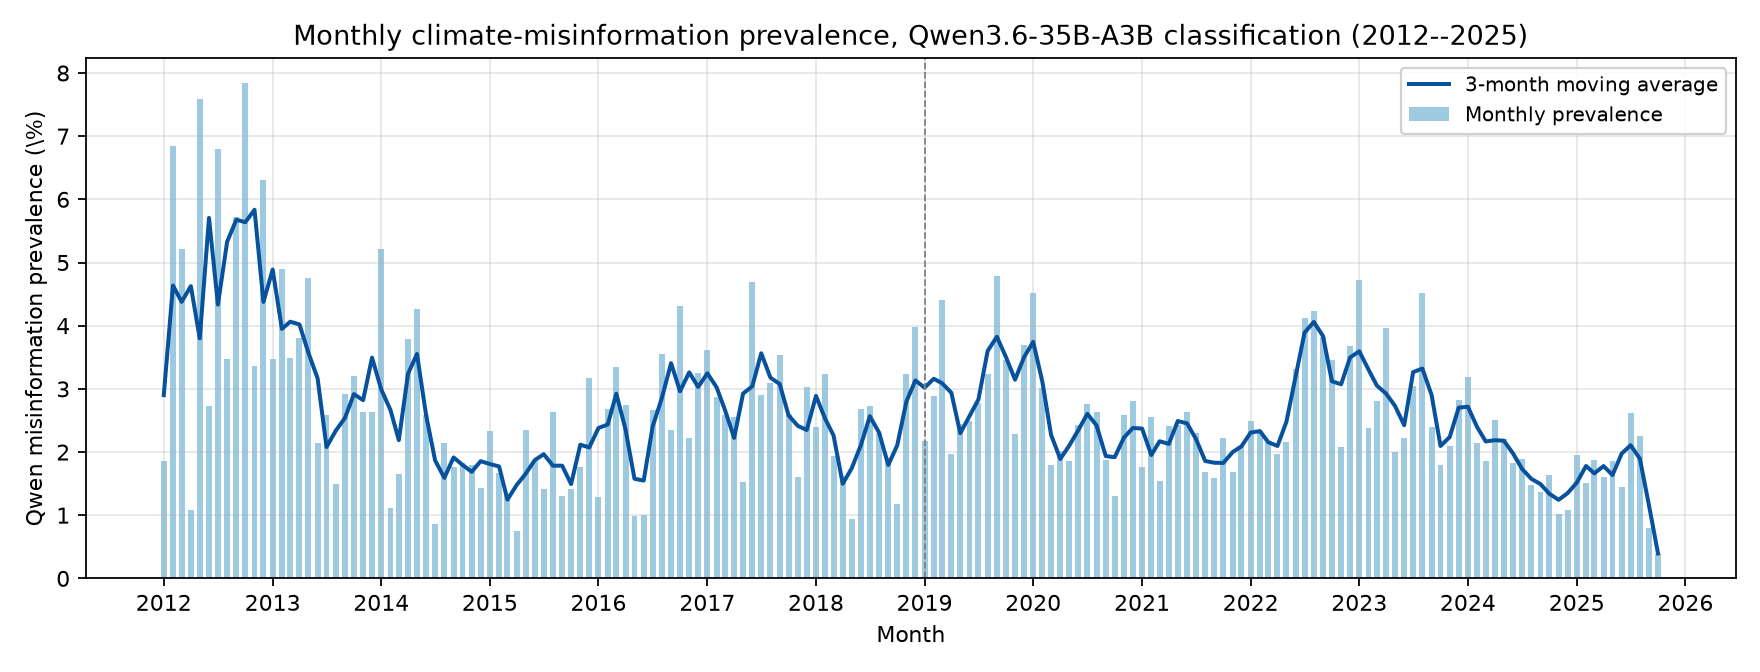
\includegraphics[width=\linewidth]{figures/fig_v2_qwen_prevalence_ts.png}
\caption{Monthly climate-misinformation prevalence in the Qwen3.6-35B-A3B classification, 2012--2025. Bars are monthly prevalence (flagged posts as a share of that month's paired posts); the solid line is a three-month moving average. The dashed line marks January 2019.}
\label{fig:qwen_prevalence_ts}
\end{figure}

\begin{figure}[!ht]
\centering
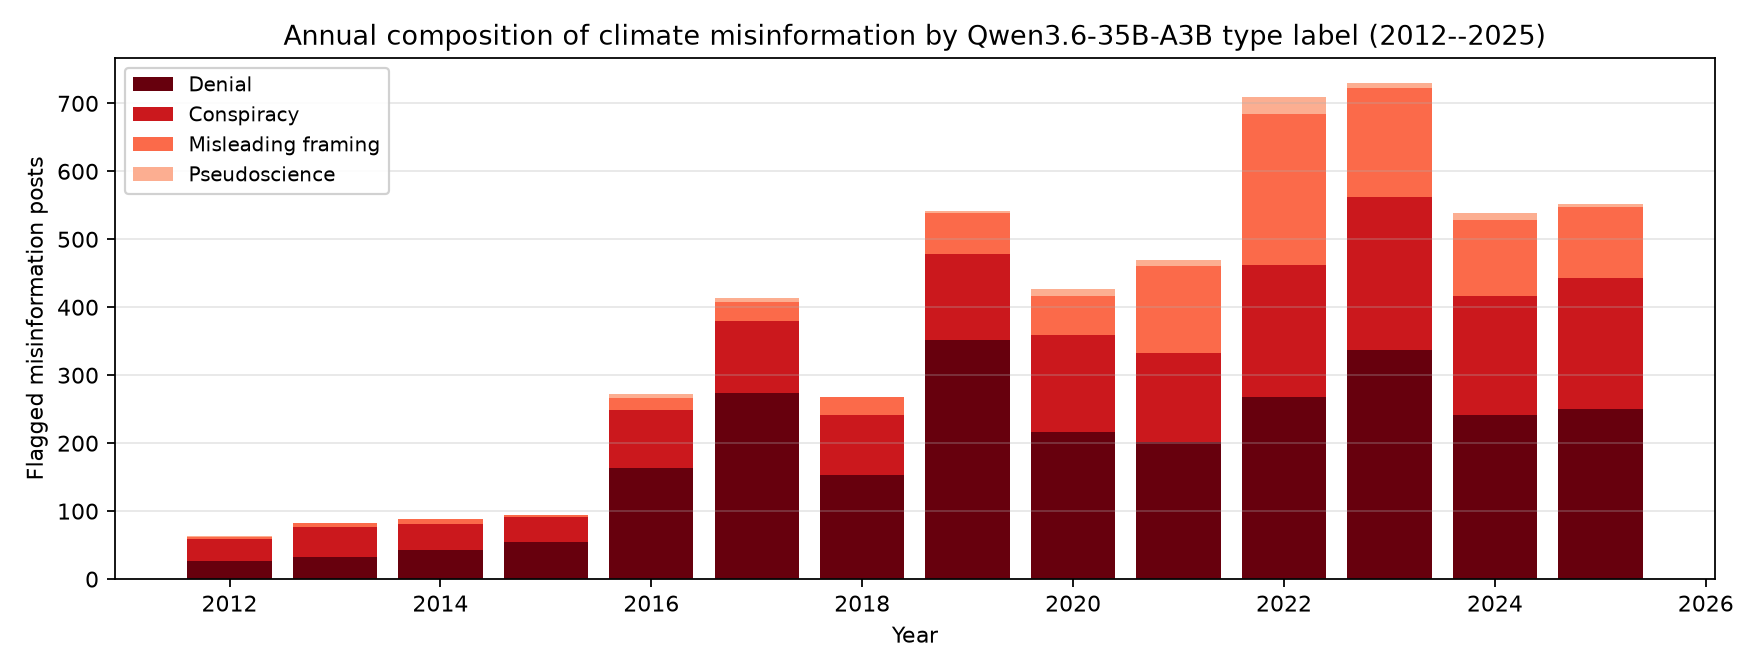
\includegraphics[width=\linewidth]{figures/fig_v2_qwen_type_composition.png}
\caption{Annual composition of Qwen-classified climate misinformation by type, 2012--2025. Denial and conspiracy framings account for the bulk of flagged content and for its post-2019 growth.}
\label{fig:qwen_type_composition}
\end{figure}

\FloatBarrier
\section{Network Structure of Misinformation Dissemination}
\label{sec:appendix_network}

I supplement the post-level corpus with an owner-based network constructed on the 150 most active and engaged post owners (pages and profiles), selected via a composite ranking weighting total engagement (40\%), misinformation post count (40\%), and overall posting activity (20\%). Two owners are connected if their monthly posting distributions correlate at $\rho \geq 0.3$ (Pearson). The largest connected component contains 142 nodes and 1{,}004 edges, with five Louvain communities (\cite{blondel2008louvain}) of community misinformation rates varying from 4.2\% to 21.7\%. The threshold captures accounts that post more during the same months, which may reflect coordinated dissemination, shared thematic interests, or common responses to COP meetings, extreme weather, or elections; the network structure should therefore be read as thematic co-occurrence rather than necessarily coordinated inauthentic behaviour (\cite{walter2020evaluating}; \cite{williams2015network}).

Three centrality measures bear on the empirical specification that follows. Eigenvector centrality is negatively correlated with the per-owner misinformation rate ($r = -0.296$, $p = 0.0004$), and degree centrality is positively correlated with the absolute misinformation count ($r = 0.218$, $p = 0.009$); betweenness centrality shows no significant association ($r = -0.068$, $p = 0.42$). The structurally central nodes disseminate proportionally lower rates of misleading content, while peripheral high-degree nodes generate larger absolute volumes. This pattern weakens, rather than supports, the prior assumption that engagement-weighting captures ``reach-amplified misinformation'': if reach were dominated by misinformation-heavy actors, eigenvector centrality should covary positively, not negatively, with misinformation rate.  Figures~\ref{fig:network_main} and~\ref{fig:centrality_misinfo} display the network and centrality scatterplots respectively.

\begin{figure}[!ht]
\centering
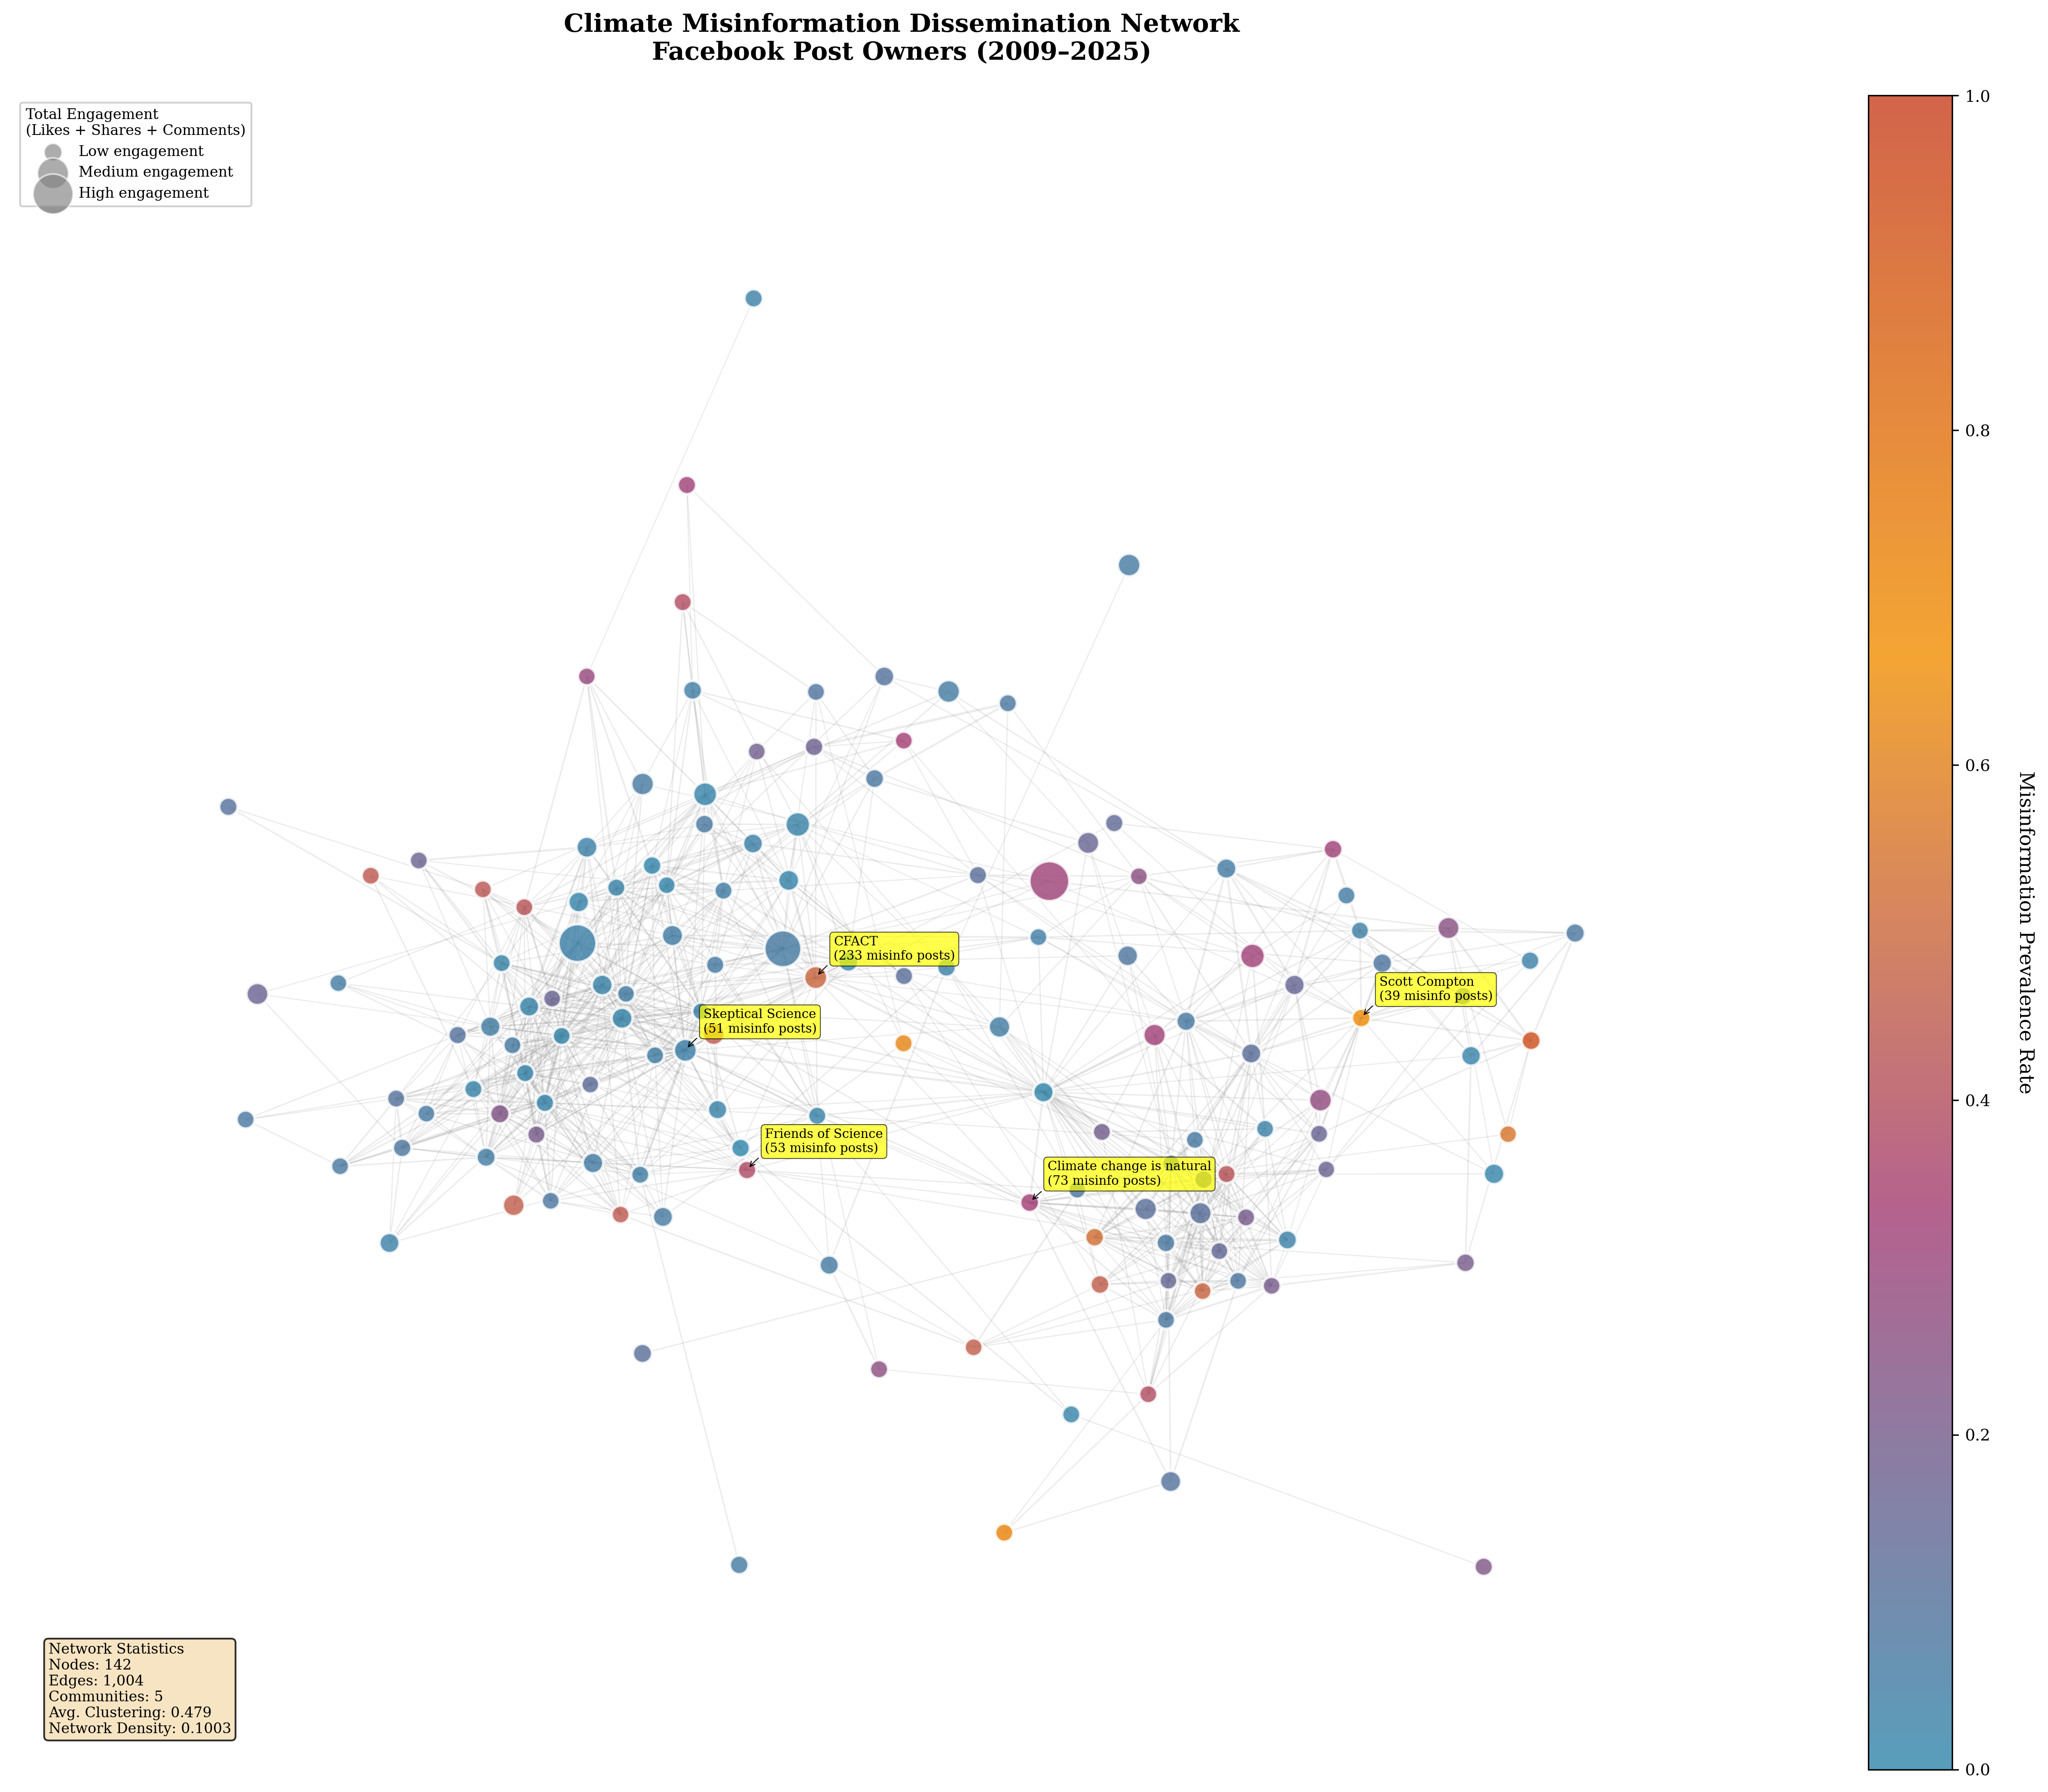
\includegraphics[width=\textwidth]{climate_misinfo_network.png}
\caption{Climate Misinformation Dissemination Network}
\label{fig:network_main}
\begin{minipage}{\textwidth}
\small
\textit{Notes:} Network graph of 142 Facebook post owners (pages/profiles) constructed from temporal posting correlations (Pearson $\rho \geq 0.3$). Node size is proportional to total engagement (likes + shares + comments). Node color indicates misinformation prevalence rate (blue = low, red = high). Edge thickness reflects correlation strength. Top 5 misinformation spreaders are labeled. Force-directed layout (Fruchterman--Reingold). Network statistics: 5 communities (Louvain), average clustering = 0.48, density = 0.10. Data source: Meta Content Library, Dec 2009-Oct 2025.
\end{minipage}
\end{figure}

\begin{figure}[!ht]
\centering
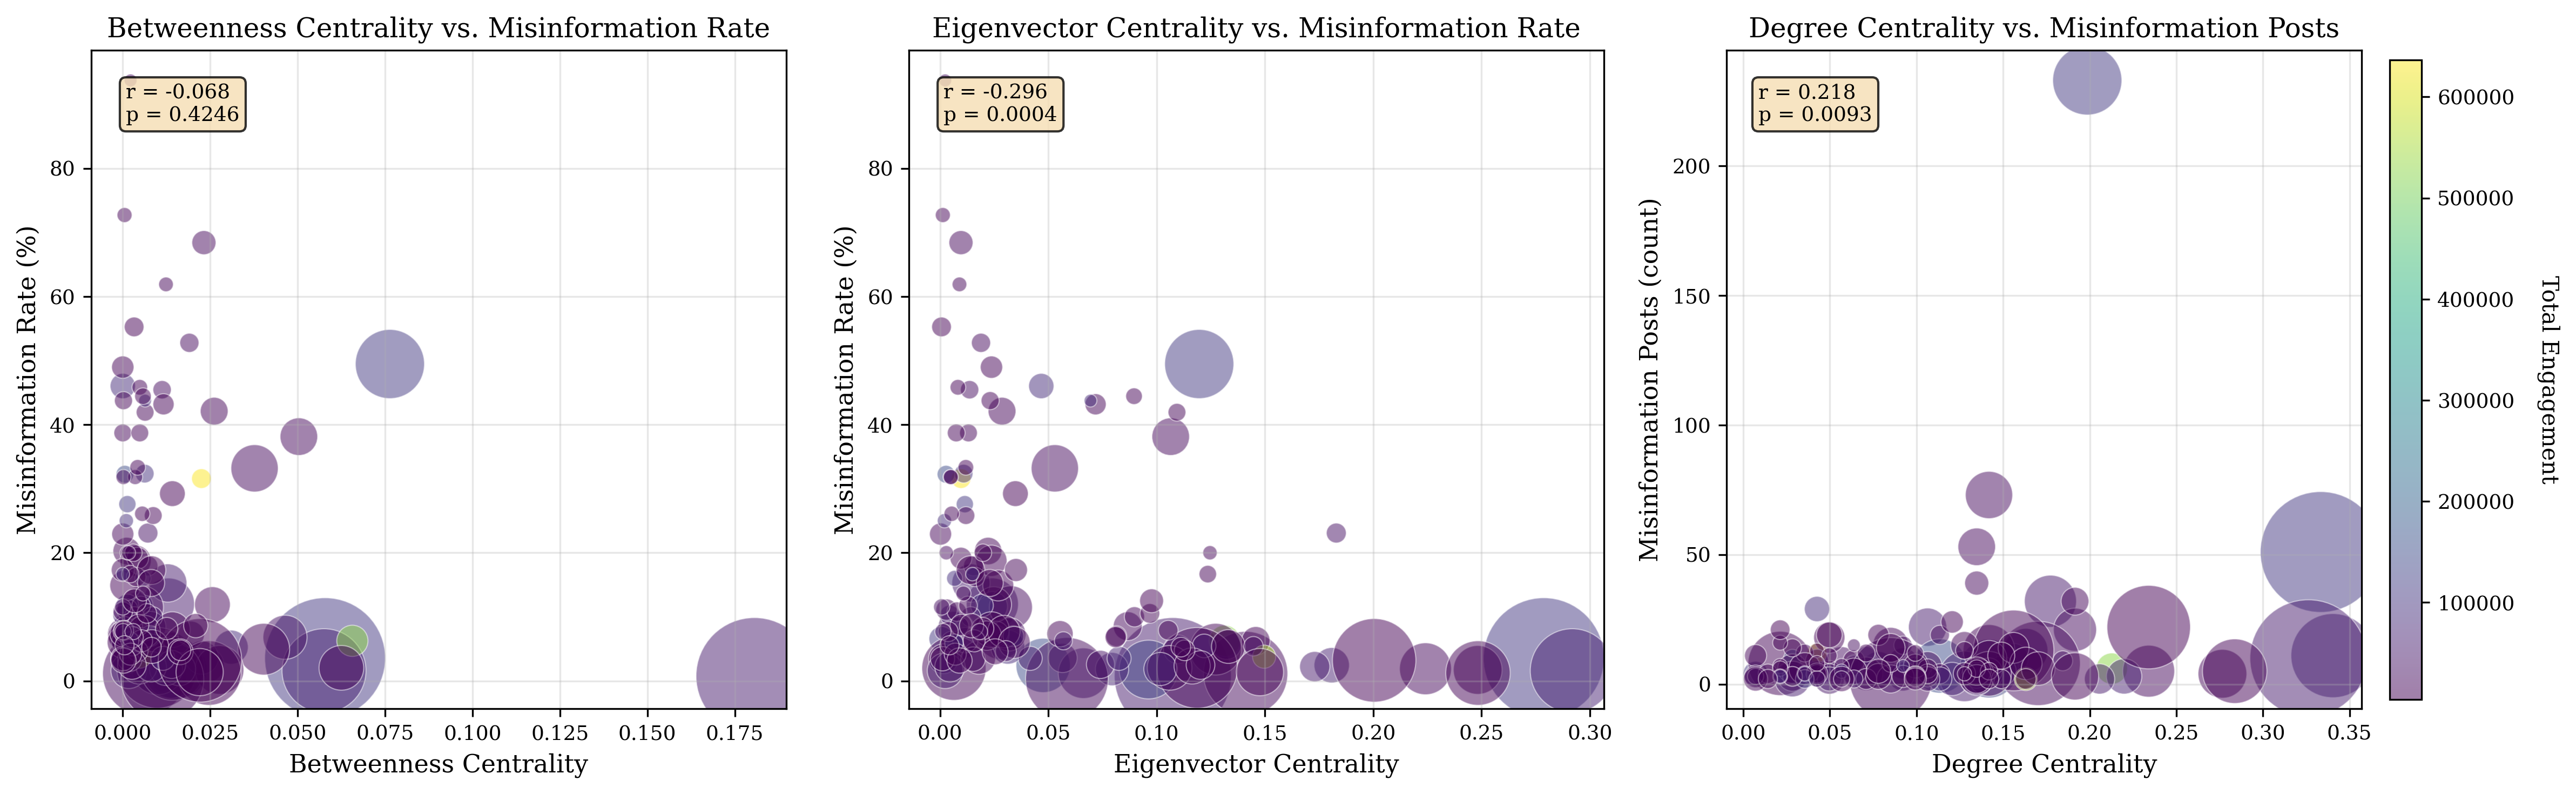
\includegraphics[width=\textwidth]{validation_test.png}
\caption{Network Centrality and Misinformation Prevalence}
\label{fig:centrality_misinfo}
\begin{minipage}{\textwidth}
\small
\textit{Notes:} Scatterplots of three centrality measures against misinformation prevalence and count. \textbf{Left panel:} Betweenness centrality vs. misinformation rate ($r = -0.068$, $p = 0.42$). \textbf{Center panel:} Eigenvector centrality vs. misinformation rate ($r = -0.296$, $p = 0.0004$). \textbf{Right panel:} Degree centrality vs. misinformation post count ($r = 0.218$, $p = 0.009$). Node size represents total posts. Color indicates total engagement. Eigenvector centrality exhibits a statistically significant negative association with misinformation rate, suggesting influential nodes spread less misinformation.
\end{minipage}
\end{figure}

\FloatBarrier
\section{Firm-Day Exposure: Descriptive Statistics and Validation}
\label{sec:firmday_validation}

This appendix reports the descriptive statistics of the firm-day misinformation-exposure
index introduced in Section~\ref{sec:LLM} and the rubric-development spot-check used to assess
the classifier's handling of satire and politically loaded but non-climate content.

\subsection{Descriptive Statistics}
Table~\ref{tab:v2_descriptive} summarises the firm-day index and its constituent scores
across the 714,227 firm-days in the climate-transition panel with at least one paired
post. The index $\mathrm{Exp}^{\text{mean}}_{i,t}$ has a mean of $0.34$ on a 0--100 scale,
a median of $0.09$, a 99th percentile of $2.73$, and a share of exactly-zero firm-days of
$44\%$. The sum variant $\mathrm{Exp}^{\text{sum}}_{i,t}$ has mean $21.85$ and 99th
percentile $171.50$; the log-transformed version $\log(1+\mathrm{Exp}^{\text{sum}}_{i,t})$
is approximately normal in shape with mean $1.80$ and 99th percentile $5.15$. The
misinformation sub-score $M^{\text{mean}}_{i,t}$ has mean $1.73$, p99 $15.60$, and a share
of exactly-zero firm-days of $41\%$, reflecting the rubric's restriction of
misinformation scoring to climate-or-energy claims. The relevance sub-score
$R^{\text{mean}}_{i,t}$ has mean $12.59$ and p99 $27.17$, with only $2\%$ of firm-days
exactly at zero, indicating that climate posts paired by date are typically at least
weakly relevant to the firm's sub-industry.

\begin{table}[htbp]
\centering
\caption{Descriptive statistics of the firm-day misinformation-exposure index (climate-transition panel, 714,227 firm-days with $\geq 1$ climate post)}
\label{tab:v2_descriptive}
\begin{threeparttable}
\footnotesize\setlength{\tabcolsep}{3pt}\begin{tabular}{p{0.39\textwidth}rrrrrr}
\toprule
Variable & Mean & SD & $p_{50}$ & $p_{90}$ & $p_{99}$ & Share zero \\
\midrule
\# climate posts paired to the firm-day & 59.900 & 49.449 & 52.000 & 127.000 & 208.000 & 0.017 \\
Mean per-post sector relevance $R^{\text{mean}}$ & 12.594 & 5.106 & 12.231 & 18.524 & 27.173 & 0.022 \\
Mean per-post climate misinformation $M^{\text{mean}}$ & 1.731 & 3.232 & 0.781 & 4.268 & 15.600 & 0.408 \\
Firm-day mean exposure $\mathrm{Exp}^{\text{mean}}$ & 0.338 & 0.715 & 0.090 & 0.971 & 2.732 & 0.442 \\
Firm-day max exposure $\mathrm{Exp}^{\text{max}}$ & 13.526 & 20.236 & 7.000 & 50.700 & 68.640 & 0.442 \\
Firm-day sum exposure $\mathrm{Exp}^{\text{sum}}$ & 21.846 & 37.661 & 7.500 & 71.250 & 171.500 & 0.442 \\
Share of posts with $M\geq 25$ & 0.020 & 0.037 & 0.009 & 0.050 & 0.167 & 0.464 \\
$\log(1+\mathrm{Exp}^{\text{sum}})$ & 1.795 & 1.758 & 2.140 & 4.280 & 5.150 & 0.442 \\
\bottomrule
\end{tabular}
\begin{tablenotes}\small
\item \textit{Notes:} Sample is firm-days in the energy panel for which at least one English-language Facebook
climate post on the same calendar date was scored against the firm's TRBC industry. ``Share zero'' is the
fraction of firm-days for which the variable evaluates to exactly 0 (typically because no posts in the day's
classification batch were judged sector-relevant or misinformation-laden).
\end{tablenotes}
\end{threeparttable}
\end{table}

Figure~\ref{fig:v2_iv_distribution} plots the distribution of the headline index and
its log-volume variant on non-zero firm-days. The mean variant has a long right tail
truncated by the bound of the 0--100 scale; the log-volume variant is more
symmetric, justifying its use in the variant Model~I specification reported in
Table~\ref{tab:v2_core}.

\begin{figure}[!ht]
\centering
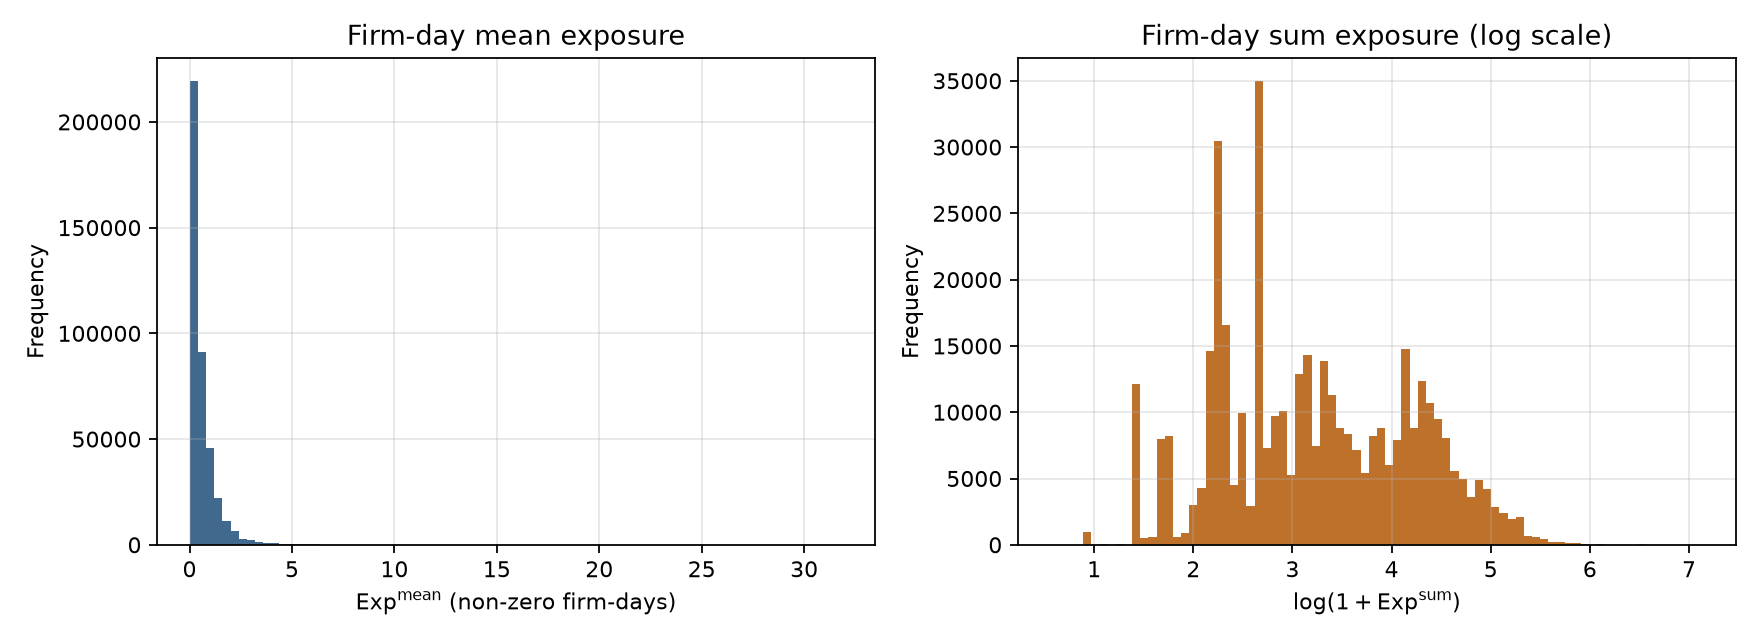
\includegraphics[width=\linewidth]{figures/fig_v2_iv_distribution.png}
\caption{Firm-day exposure distribution. Left panel: $\mathrm{Exp}^{\text{mean}}_{i,t}$
on non-zero firm-days. Right panel: $\log(1+\mathrm{Exp}^{\text{sum}}_{i,t})$.}
\label{fig:v2_iv_distribution}
\end{figure}

\subsection{Classifier Validation}
The classifier was assessed during rubric development using a spot-check of the first 2,000 (post,
sub-industry) judgments. Two qualitative findings shaped the final rubric. First, a
default rubric (``score climate misinformation on a continuous 0--100 scale'')
over-scored politically charged but non-climate content. Anti-vaccine conspiracy
posts, antisemitic content about EU politicians, and electoral-fraud posts that
happened to be paired to climate sub-industries by calendar date received high
misinformation scores under the default rubric despite making no empirical claims
about climate or energy. The headline composite $\mathrm{Exp}_{p,s}=R_{p,s}\cdot
M_{p,s}/100$ partially neutralised this leakage because relevance scores on
sector-irrelevant content were low, but the misinformation sub-score itself was
contaminated. The final rubric (Section~\ref{sec:LLM}) explicitly restricts
misinformation scoring to climate-or-energy claims, and a re-run of the spot-check
under the final rubric produced misinformation scores of zero on the politically
charged but non-climate items.

Second, sarcastic and parodic content that mocked climate denial received high
misinformation scores under the default rubric. A representative example begins
``MDPI, the predatory journal of which nothing can be believed, according to
Facebook climate experts, recently published a dubious study on anthropogenic
warming\ldots'' and ends with the parody credit ``A DONT BELIEVE EVERYTHING YOU
READ PRODUCTION''. The default rubric scored this post at $M_{p,s}=95$ with the
type label ``denial''; the final rubric, which includes an explicit instruction to
treat satire and parody as not-misinformation, scores it at $M_{p,s}=0$ with the
rationale ``satirical parody mocking climate denialism, not a sincere assertion of
false claims''. Both rubric refinements were committed to the spec before the
production run, and the production run used the final rubric.

\subsection{Within-Classifier Relevance Checks}
The natural relevance check compares highly sector-relevant posts with those assigned a low relevance score. A high-relevance conditional mean and its contribution to the all-post mean are different regressors. If $H_p=1\{R_{p,s}\geq c\}$, $q^H$ is the qualifying-post share and $\bar e^H$ its mean exposure, then $C^H=q^H\bar e^H$ and $E=C^H+C^L$. This decomposition permits different coefficient signs without an algebraic contradiction. It does not establish the empirical cause of a difference. An empty qualifying subset has an undefined conditional mean, whereas its all-post contribution is zero.

The fixed score files and saved daily index are available, but the internal post-ID/date crosswalk required to reaggregate thresholded daily subsets is not distributed. The supplied aggregation code preserves missing conditional means, reports common-denominator contributions at four relevance thresholds and fails explicitly if the crosswalk is absent. No irrelevant-post placebo is treated as newly reproduced support for specificity. The completed mean-relevance, misinformation-score, positive-content and volume-adjusted regressions are reported in Table~\ref{tab:variants}; these remain internal measurement checks, not independent validation of classifier accuracy.

\FloatBarrier
\section{Heterogeneity and Interaction Checks}
\label{sec:appendix_heterogeneity}
\subsection{Sector and Listing-Market Sensitivity}
\label{sec:results_signflip}
The leave-out comparisons retain the fully conditional model and the full sample's tail caps while omitting each energy sub-industry in turn. Table~\ref{tab:leaveout} also reports omission of the three largest listing markets. This assesses whether a particular sector or market supplies the fitted association without changing financial tail treatment within every subsample. All use the completed saved estimates.
\begin{table}[htbp]
\centering
\caption{Leave-out diagnostics with fixed full-sample tail caps}
\label{tab:leaveout}
\begin{minipage}{\linewidth}
\footnotesize
\setlength{\tabcolsep}{4pt}
\begingroup\centering
\begin{tabular}{p{0.51\linewidth}rrr}
\toprule
Omitted sector or market & Coefficient & SE & $p$ \\
\midrule
Coal & -0.0013 & 0.0031 & 0.698 \\
Integrated Oil \& Gas & -0.0013 & 0.0026 & 0.635 \\
Oil \& Gas Drilling & -0.0020 & 0.0022 & 0.386 \\
Oil \& Gas Exploration and Production & -0.0010 & 0.0026 & 0.719 \\
Oil \& Gas Refining and Marketing & 0.0000 & 0.0027 & 0.992 \\
Oil \& Gas Transportation Services & -0.0015 & 0.0025 & 0.572 \\
Oil Related Services and Equipment & -0.0025 & 0.0021 & 0.266 \\
Renewable Energy Equipment \& Services & -0.0028 & 0.0025 & 0.296 \\
Renewable Fuels & -0.0006 & 0.0021 & 0.797 \\
Market: Mainland China & -0.0023 & 0.0032 & 0.482 \\
Market: Indonesia & 0.0002 & 0.0010 & 0.838 \\
Market: United States & -0.0020 & 0.0027 & 0.481 \\
\bottomrule
\end{tabular}\par\endgroup
\par\vspace{0.5em}\footnotesize All specifications retain the principal controls and fixed effects. Leaving out a sector leaves eight sector clusters. The full principal sample supplies tail caps; they are not recomputed within each leave-out sample.
\end{minipage}
\end{table}

Across sector omissions, coefficients range from approximately $-0.0028$ to $0.0000$. The intervals remain imprecise, and the table does not establish a robust positive coefficient under the fully conditional design. These checks identify the scope of that null result, rather than overwrite the positive association under broader controls. Figure~\ref{fig:leaveout} displays the sector comparisons.
\begin{figure}[htbp]\centering
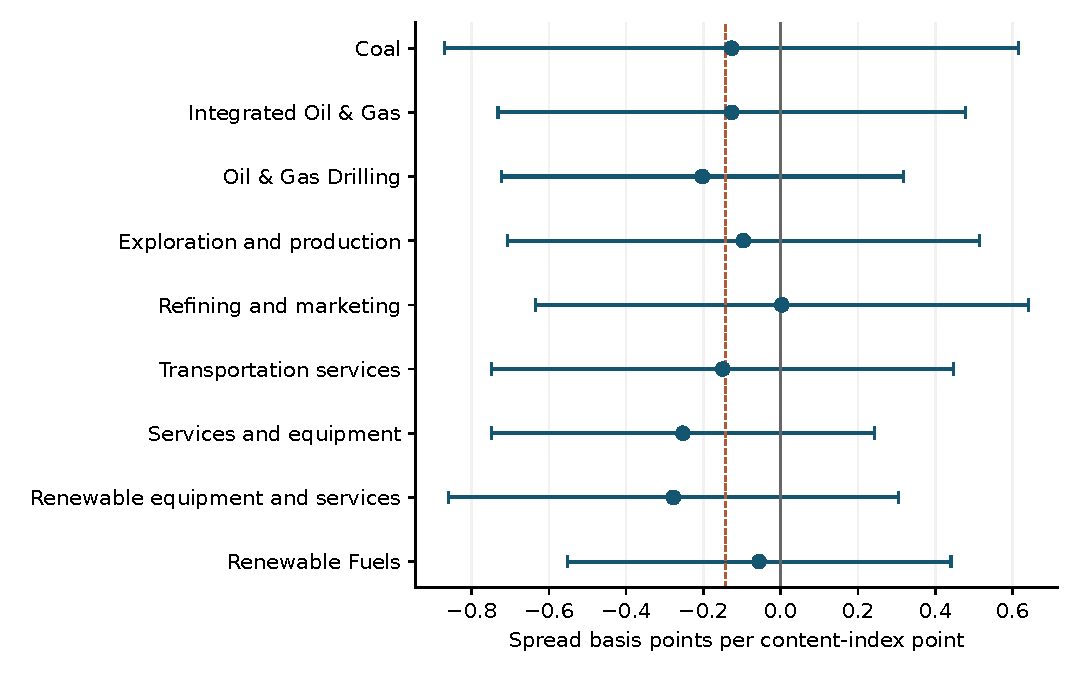
\includegraphics[width=\linewidth]{figures/leave_sector_out.pdf}
\caption{Exposure coefficients after omitting one sector at a time, using the fully conditional model and fixed full-sample tail caps. Bars are approximate 95\% sector/date-clustered intervals, with seven reference degrees of freedom.}
\label{fig:leaveout}\end{figure}
\subsection{Temporal Interaction}
\label{sec:results_triple}
The completed temporal check interacts the exposure index with a post-2019 indicator while retaining security, market-day and sector-month effects and prior-session financial controls. The interaction is $-0.0019$ with $p=0.687$. This directly tests a slope difference. It does not show a strengthened spread association after 2019, even though the amount and sector distribution of classified content change. Stored region-group interactions are not interpreted as language-market effects because the input groups do not map cleanly to actual listing markets.

\FloatBarrier
\section{Additional Specification and Inference Checks}
\label{sec:appendix_robustness}
\begin{table}[htbp]
\centering
\caption{Alternative inference for the principal coefficient}
\label{tab:inference}
\begin{minipage}{\linewidth}
\small
\setlength{\tabcolsep}{4pt}
\begingroup\centering
\begin{tabular}{p{0.57\linewidth}rr}
\toprule
Reference calculation & SE & $p$ \\
\midrule
Security/date clusters & 0.00108 & 0.188 \\
Sector/date clusters & 0.00220 & 0.533 \\
Date-score HAC, bandwidth 5 & 0.00225 & 0.524 \\
Date-score HAC, bandwidth 20 & 0.00223 & 0.521 \\
Date-score HAC, bandwidth 60 & 0.00201 & 0.476 \\
Sector score signs & --- & 0.512 \\
\bottomrule
\end{tabular}\par\endgroup
\par\vspace{0.5em}\footnotesize The coefficient and observations are identical in every row. Sector/date clustering has nine sectors. HAC uses ordered observed dates and a normal reference. Score signs enumerate 512 combinations and require independent symmetric sector scores; this is a diagnostic, not exact randomization inference.
\end{minipage}
\end{table}

\begin{table}[htbp]
\centering
\caption{Alternative content measures and attention adjustment}
\label{tab:variants}
\begin{minipage}{\linewidth}
\small
\setlength{\tabcolsep}{4pt}
\begin{tabular}{p{0.48\linewidth}rrr}
\toprule
Content regressor & Coefficient & SE & $p$ \\
\midrule
Mean composite & -0.0014 & 0.0022 & 0.533 \\
Log of one plus composite sum & 0.0002 & 0.0010 & 0.820 \\
Mean misinformation score & 0.0010 & 0.0013 & 0.470 \\
Mean relevance score & -0.0002 & 0.0004 & 0.644 \\
Share with misinformation at least 25 & 0.0338 & 0.0897 & 0.716 \\
Positive composite indicator & -0.0036 & 0.0040 & 0.398 \\
Composite with volume and relevance controls & -0.0013 & 0.0023 & 0.591 \\
\bottomrule
\end{tabular}
\par\vspace{0.5em}\footnotesize Principal controls and fixed effects throughout. Regressor units differ across rows; raw coefficient sizes are not comparable. The final row adds log one plus post count and mean relevance jointly. Sector/date inference.
\end{minipage}
\end{table}

\begin{table}[htbp]
\centering
\caption{Outcome, sample, and timing sensitivity}
\label{tab:sensitivity}
\begin{minipage}{\linewidth}
\footnotesize
\setlength{\tabcolsep}{4pt}
\begin{tabular}{p{0.40\linewidth}rrrr}
\toprule
Specification & Coefficient & SE & $p$ & N \\
\midrule
No financial controls & -0.0012 & 0.0017 & 0.492 & 485,800 \\
Unwinsorized spread and controls & -0.0086 & 0.0048 & 0.109 & 485,800 \\
Log spread & 0.0035 & 0.0020 & 0.122 & 485,800 \\
Matched-post dates only & -0.0014 & 0.0022 & 0.556 & 485,332 \\
Previous-session content & -0.0010 & 0.0022 & 0.652 & 485,759 \\
VWAP-midpoint percentage gap & 0.0010 & 0.0033 & 0.760 & 485,798 \\
\bottomrule
\end{tabular}
\par\vspace{0.5em}\footnotesize Unless stated otherwise the outcome is a percentage-point spread. Log spread and the VWAP gap have different units/interpretations. No gap outcome is interpreted as transaction price impact. Sector/date inference.
\end{minipage}
\end{table}

\begin{table}[htbp]
\centering
\caption{Financial control definitions and tail caps}
\label{tab:controls}
\begin{minipage}{\linewidth}
\small
\setlength{\tabcolsep}{4pt}
\begingroup\centering
\begin{tabular}{p{0.55\linewidth}rr}
\toprule
Variable & Lower cap & Upper cap \\
\midrule
Quoted spread, percent & 0.0085 & 7.5381 \\
Prior log one plus volume & 7.9014 & 19.3589 \\
Prior log market capitalization & 20.1426 & 31.9419 \\
Prior range as percent of close & 0.0000 & 14.7036 \\
\bottomrule
\end{tabular}\par\endgroup
\par\vspace{0.5em}\footnotesize Principal sample first and ninety-ninth percentile caps. Exposure scores are not capped.
\end{minipage}
\end{table}

The nine-sector structure motivates comparing sector/date clustering with date-score HAC and the sector score-sign diagnostic. Their assumptions and finite-sample limits are set out in the supplementary material. The full set of completed coefficient estimates is retained, including numerical warnings. In the attention-adjusted model the post-volume control has an undefined sector/date standard error; the exposure coefficient and all coefficients in the fully conditional model have finite reported uncertainty. The absence of a robust positive coefficient in the saturated models limits an independent daily misinformation interpretation without erasing the positive broader association documented in the main text.

\FloatBarrier
\section{Summary}

The appendix consolidates the descriptive and diagnostic evidence behind the paper's design. The corpus tables document the scale, heterogeneity, and engagement structure of the Facebook data; the network section maps the dissemination structure of the most active post owners. Together they document how the explanatory variable is constructed from variation in post volume, engagement, and timing.

The financial and exposure sections document coverage, composition and the construction of the exposure index: its distributional properties, the rubric-development spot-check, and the distinction between content availability and observed investor attention. The conditional-mean decomposition explains why relevance subsets need not reproduce the all-post association, while the empirical checks distinguish market-day conditions from sector-month conditions. Read together, the appendix connects the competing-liquidity framework in Section~\ref{sec:theory} to the positive associations and their empirical boundaries in Section~\ref{sec:results}.

\end{document}
